\documentclass[twoside]{book}

% Packages required by doxygen
\usepackage{calc}
\usepackage{doxygen}
\usepackage{graphicx}
\usepackage[utf8]{inputenc}
\usepackage{makeidx}
\usepackage{multicol}
\usepackage{multirow}
\usepackage{textcomp}
\usepackage[table]{xcolor}

% Font selection
\usepackage[T1]{fontenc}
\usepackage{mathptmx}
\usepackage[scaled=.90]{helvet}
\usepackage{courier}
\usepackage{amssymb}
\usepackage{sectsty}
\renewcommand{\familydefault}{\sfdefault}
\allsectionsfont{%
  \fontseries{bc}\selectfont%
  \color{darkgray}%
}
\renewcommand{\DoxyLabelFont}{%
  \fontseries{bc}\selectfont%
  \color{darkgray}%
}

% Page & text layout
\usepackage{geometry}
\geometry{%
  a4paper,%
  top=2.5cm,%
  bottom=2.5cm,%
  left=2.5cm,%
  right=2.5cm%
}
\tolerance=750
\hfuzz=15pt
\hbadness=750
\setlength{\emergencystretch}{15pt}
\setlength{\parindent}{0cm}
\setlength{\parskip}{0.2cm}
\makeatletter
\renewcommand{\paragraph}{%
  \@startsection{paragraph}{4}{0ex}{-1.0ex}{1.0ex}{%
    \normalfont\normalsize\bfseries\SS@parafont%
  }%
}
\renewcommand{\subparagraph}{%
  \@startsection{subparagraph}{5}{0ex}{-1.0ex}{1.0ex}{%
    \normalfont\normalsize\bfseries\SS@subparafont%
  }%
}
\makeatother

% Headers & footers
\usepackage{fancyhdr}
\pagestyle{fancyplain}
\fancyhead[LE]{\fancyplain{}{\bfseries\thepage}}
\fancyhead[CE]{\fancyplain{}{}}
\fancyhead[RE]{\fancyplain{}{\bfseries\leftmark}}
\fancyhead[LO]{\fancyplain{}{\bfseries\rightmark}}
\fancyhead[CO]{\fancyplain{}{}}
\fancyhead[RO]{\fancyplain{}{\bfseries\thepage}}
\fancyfoot[LE]{\fancyplain{}{}}
\fancyfoot[CE]{\fancyplain{}{}}
\fancyfoot[RE]{\fancyplain{}{\bfseries\scriptsize Generated on Tue Sep 24 2013 19:22:44 for My Project by Doxygen }}
\fancyfoot[LO]{\fancyplain{}{\bfseries\scriptsize Generated on Tue Sep 24 2013 19:22:44 for My Project by Doxygen }}
\fancyfoot[CO]{\fancyplain{}{}}
\fancyfoot[RO]{\fancyplain{}{}}
\renewcommand{\footrulewidth}{0.4pt}
\renewcommand{\chaptermark}[1]{%
  \markboth{#1}{}%
}
\renewcommand{\sectionmark}[1]{%
  \markright{\thesection\ #1}%
}

% Indices & bibliography
\usepackage{natbib}
\usepackage[titles]{tocloft}
\setcounter{tocdepth}{3}
\setcounter{secnumdepth}{5}
\makeindex

% Hyperlinks (required, but should be loaded last)
\usepackage{ifpdf}
\ifpdf
  \usepackage[pdftex,pagebackref=true]{hyperref}
\else
  \usepackage[ps2pdf,pagebackref=true]{hyperref}
\fi
\hypersetup{%
  colorlinks=true,%
  linkcolor=blue,%
  citecolor=blue,%
  unicode%
}

% Custom commands
\newcommand{\clearemptydoublepage}{%
  \newpage{\pagestyle{empty}\cleardoublepage}%
}


%===== C O N T E N T S =====

\begin{document}

% Titlepage & ToC
\hypersetup{pageanchor=false}
\pagenumbering{roman}
\begin{titlepage}
\vspace*{7cm}
\begin{center}%
{\Large My Project }\\
\vspace*{1cm}
{\large Generated by Doxygen 1.8.4}\\
\vspace*{0.5cm}
{\small Tue Sep 24 2013 19:22:44}\\
\end{center}
\end{titlepage}
\clearemptydoublepage
\tableofcontents
\clearemptydoublepage
\pagenumbering{arabic}
\hypersetup{pageanchor=true}

%--- Begin generated contents ---
\chapter{R\-E\-A\-D\-M\-E}
\label{md_README}
\hypertarget{md_README}{}
D\-E\-P\-E\-N\-D\-E\-N\-C\-Y\-:
\begin{DoxyItemize}
\item flask
\item gevent
\item geventwebsocket
\item greenlet
\item rsa 
\end{DoxyItemize}
\chapter{Namespace Index}
\section{Namespace List}
Here is a list of all documented namespaces with brief descriptions\-:\begin{DoxyCompactList}
\item\contentsline{section}{\hyperlink{namespaceweb_1_1database}{web.\-database} }{\pageref{namespaceweb_1_1database}}{}
\item\contentsline{section}{\hyperlink{namespaceweb_1_1_simulate___class}{web.\-Simulate\-\_\-\-Class} }{\pageref{namespaceweb_1_1_simulate___class}}{}
\item\contentsline{section}{\hyperlink{namespaceweb_1_1user}{web.\-user} }{\pageref{namespaceweb_1_1user}}{}
\end{DoxyCompactList}

\chapter{Hierarchical Index}
\section{Class Hierarchy}
This inheritance list is sorted roughly, but not completely, alphabetically\-:\begin{DoxyCompactList}
\item \contentsline{section}{web.\-websocket.\-apis}{\pageref{classweb_1_1websocket_1_1apis}}{}
\item \contentsline{section}{Base}{\pageref{class_base}}{}
\begin{DoxyCompactList}
\item \contentsline{section}{m\-R\-N\-A}{\pageref{classm_r_n_a}}{}
\item \contentsline{section}{Protein}{\pageref{class_protein}}{}
\end{DoxyCompactList}
\item \contentsline{section}{D\-N\-A}{\pageref{class_d_n_a}}{}
\item \contentsline{section}{web.\-Simulate\-\_\-\-Class.\-D\-N\-A\-\_\-\-Simulate}{\pageref{classweb_1_1_simulate___class_1_1_d_n_a___simulate}}{}
\item \contentsline{section}{web.\-encrypt.\-Encrypt}{\pageref{classweb_1_1encrypt_1_1_encrypt}}{}
\item Exception\begin{DoxyCompactList}
\item \contentsline{section}{web.\-Simulate\-\_\-\-Class.\-Illegal\-Setting}{\pageref{classweb_1_1_simulate___class_1_1_illegal_setting}}{}
\item \contentsline{section}{web.\-Simulate\-\_\-\-Class.\-Invalid\-Parameter}{\pageref{classweb_1_1_simulate___class_1_1_invalid_parameter}}{}
\end{DoxyCompactList}
\item \contentsline{section}{web.\-modeling.\-modeling}{\pageref{classweb_1_1modeling_1_1modeling}}{}
\item \contentsline{section}{web.\-Simulate\-\_\-\-Class.\-m\-R\-N\-A\-\_\-\-Simulate}{\pageref{classweb_1_1_simulate___class_1_1m_r_n_a___simulate}}{}
\item \contentsline{section}{web.\-Simulate\-\_\-\-Class.\-Protein\-\_\-\-Simulate}{\pageref{classweb_1_1_simulate___class_1_1_protein___simulate}}{}
\item \contentsline{section}{web.\-component\-\_\-union.\-R\-F\-C10}{\pageref{classweb_1_1component__union_1_1_r_f_c10}}{}
\item \contentsline{section}{web.\-component\-\_\-union.\-R\-F\-C20}{\pageref{classweb_1_1component__union_1_1_r_f_c20}}{}
\item \contentsline{section}{web.\-component\-\_\-union.\-R\-F\-C21}{\pageref{classweb_1_1component__union_1_1_r_f_c21}}{}
\item \contentsline{section}{web.\-component\-\_\-union.\-R\-F\-C23}{\pageref{classweb_1_1component__union_1_1_r_f_c23}}{}
\item \contentsline{section}{web.\-component\-\_\-union.\-R\-F\-C25}{\pageref{classweb_1_1component__union_1_1_r_f_c25}}{}
\item \contentsline{section}{web.\-shared\-File.\-shared\-Files}{\pageref{classweb_1_1shared_file_1_1shared_files}}{}
\item \contentsline{section}{web.\-database.\-Sqlite\-Database}{\pageref{classweb_1_1database_1_1_sqlite_database}}{}
\item \contentsline{section}{web.\-modeling2.\-Struct1\-\_\-\-S\-Y\-S\-U\-\_\-\-Software}{\pageref{classweb_1_1modeling2_1_1_struct1___s_y_s_u___software}}{}
\item \contentsline{section}{web.\-modeling2.\-Struct2\-\_\-\-S\-Y\-S\-U\-\_\-\-Software}{\pageref{classweb_1_1modeling2_1_1_struct2___s_y_s_u___software}}{}
\item \contentsline{section}{web.\-modeling2.\-Struct3\-\_\-\-S\-Y\-S\-U\-\_\-\-Software}{\pageref{classweb_1_1modeling2_1_1_struct3___s_y_s_u___software}}{}
\item \contentsline{section}{web.\-xml\-Parse.\-xml\-Biobrick}{\pageref{classweb_1_1xml_parse_1_1xml_biobrick}}{}
\end{DoxyCompactList}

\chapter{Class Index}
\section{Class List}
Here are the classes, structs, unions and interfaces with brief descriptions\-:\begin{DoxyCompactList}
\item\contentsline{section}{\hyperlink{classweb_1_1websocket_1_1apis}{web.\-websocket.\-apis} }{\pageref{classweb_1_1websocket_1_1apis}}{}
\item\contentsline{section}{\hyperlink{class_base}{Base} }{\pageref{class_base}}{}
\item\contentsline{section}{\hyperlink{class_d_n_a}{D\-N\-A} }{\pageref{class_d_n_a}}{}
\item\contentsline{section}{\hyperlink{classweb_1_1_simulate___class_1_1_d_n_a___simulate}{web.\-Simulate\-\_\-\-Class.\-D\-N\-A\-\_\-\-Simulate} \\*\subsubsection*{calculating \hyperlink{class_d_n_a}{D\-N\-A} simulation result }}{\pageref{classweb_1_1_simulate___class_1_1_d_n_a___simulate}}{}
\item\contentsline{section}{\hyperlink{classweb_1_1encrypt_1_1_encrypt}{web.\-encrypt.\-Encrypt} \\*\subsubsection*{the class that can provide R\-S\-A method }}{\pageref{classweb_1_1encrypt_1_1_encrypt}}{}
\item\contentsline{section}{\hyperlink{classweb_1_1_simulate___class_1_1_illegal_setting}{web.\-Simulate\-\_\-\-Class.\-Illegal\-Setting} }{\pageref{classweb_1_1_simulate___class_1_1_illegal_setting}}{}
\item\contentsline{section}{\hyperlink{classweb_1_1_simulate___class_1_1_invalid_parameter}{web.\-Simulate\-\_\-\-Class.\-Invalid\-Parameter} }{\pageref{classweb_1_1_simulate___class_1_1_invalid_parameter}}{}
\item\contentsline{section}{\hyperlink{classweb_1_1modeling_1_1modeling}{web.\-modeling.\-modeling} }{\pageref{classweb_1_1modeling_1_1modeling}}{}
\item\contentsline{section}{\hyperlink{classm_r_n_a}{m\-R\-N\-A} }{\pageref{classm_r_n_a}}{}
\item\contentsline{section}{\hyperlink{classweb_1_1_simulate___class_1_1m_r_n_a___simulate}{web.\-Simulate\-\_\-\-Class.\-m\-R\-N\-A\-\_\-\-Simulate} \\*Calculating \hyperlink{classm_r_n_a}{m\-R\-N\-A} simulation result }{\pageref{classweb_1_1_simulate___class_1_1m_r_n_a___simulate}}{}
\item\contentsline{section}{\hyperlink{class_protein}{Protein} }{\pageref{class_protein}}{}
\item\contentsline{section}{\hyperlink{classweb_1_1_simulate___class_1_1_protein___simulate}{web.\-Simulate\-\_\-\-Class.\-Protein\-\_\-\-Simulate} }{\pageref{classweb_1_1_simulate___class_1_1_protein___simulate}}{}
\item\contentsline{section}{\hyperlink{classweb_1_1component__union_1_1_r_f_c10}{web.\-component\-\_\-union.\-R\-F\-C10} }{\pageref{classweb_1_1component__union_1_1_r_f_c10}}{}
\item\contentsline{section}{\hyperlink{classweb_1_1component__union_1_1_r_f_c20}{web.\-component\-\_\-union.\-R\-F\-C20} }{\pageref{classweb_1_1component__union_1_1_r_f_c20}}{}
\item\contentsline{section}{\hyperlink{classweb_1_1component__union_1_1_r_f_c21}{web.\-component\-\_\-union.\-R\-F\-C21} }{\pageref{classweb_1_1component__union_1_1_r_f_c21}}{}
\item\contentsline{section}{\hyperlink{classweb_1_1component__union_1_1_r_f_c23}{web.\-component\-\_\-union.\-R\-F\-C23} }{\pageref{classweb_1_1component__union_1_1_r_f_c23}}{}
\item\contentsline{section}{\hyperlink{classweb_1_1component__union_1_1_r_f_c25}{web.\-component\-\_\-union.\-R\-F\-C25} }{\pageref{classweb_1_1component__union_1_1_r_f_c25}}{}
\item\contentsline{section}{\hyperlink{classweb_1_1shared_file_1_1shared_files}{web.\-shared\-File.\-shared\-Files} \\*\subsubsection*{the class that have wrap the method about controling the shared files }}{\pageref{classweb_1_1shared_file_1_1shared_files}}{}
\item\contentsline{section}{\hyperlink{classweb_1_1database_1_1_sqlite_database}{web.\-database.\-Sqlite\-Database} }{\pageref{classweb_1_1database_1_1_sqlite_database}}{}
\item\contentsline{section}{\hyperlink{classweb_1_1modeling2_1_1_struct1___s_y_s_u___software}{web.\-modeling2.\-Struct1\-\_\-\-S\-Y\-S\-U\-\_\-\-Software} }{\pageref{classweb_1_1modeling2_1_1_struct1___s_y_s_u___software}}{}
\item\contentsline{section}{\hyperlink{classweb_1_1modeling2_1_1_struct2___s_y_s_u___software}{web.\-modeling2.\-Struct2\-\_\-\-S\-Y\-S\-U\-\_\-\-Software} }{\pageref{classweb_1_1modeling2_1_1_struct2___s_y_s_u___software}}{}
\item\contentsline{section}{\hyperlink{classweb_1_1modeling2_1_1_struct3___s_y_s_u___software}{web.\-modeling2.\-Struct3\-\_\-\-S\-Y\-S\-U\-\_\-\-Software} }{\pageref{classweb_1_1modeling2_1_1_struct3___s_y_s_u___software}}{}
\item\contentsline{section}{\hyperlink{classweb_1_1xml_parse_1_1xml_biobrick}{web.\-xml\-Parse.\-xml\-Biobrick} \\*\subsubsection*{the class that can parse a xml to a biobrick object }}{\pageref{classweb_1_1xml_parse_1_1xml_biobrick}}{}
\end{DoxyCompactList}

\chapter{File Index}
\section{File List}
Here is a list of all documented files with brief descriptions\-:\begin{DoxyCompactList}
\item\contentsline{section}{{\bfseries graph.\-h} }{\pageref{graph_8h}}{}
\item\contentsline{section}{\hyperlink{_simulate___class_8py}{Simulate\-\_\-\-Class.\-py} \\*Calculate Simulation data }{\pageref{_simulate___class_8py}}{}
\end{DoxyCompactList}

\chapter{Namespace Documentation}
\hypertarget{namespaceweb_1_1database}{\section{web.\-database Namespace Reference}
\label{namespaceweb_1_1database}\index{web.\-database@{web.\-database}}
}
\subsection*{Classes}
\begin{DoxyCompactItemize}
\item 
class \hyperlink{classweb_1_1database_1_1_sqlite_database}{Sqlite\-Database}
\end{DoxyCompactItemize}
\subsection*{Variables}
\begin{DoxyCompactItemize}
\item 
\hypertarget{namespaceweb_1_1database_a8ee68d73d9fa5cb7d602355fb7ce0b92}{tuple {\bfseries sql} = \hyperlink{classweb_1_1database_1_1_sqlite_database}{Sqlite\-Database}()}\label{namespaceweb_1_1database_a8ee68d73d9fa5cb7d602355fb7ce0b92}

\end{DoxyCompactItemize}


\subsection{Detailed Description}
\begin{DoxyVerb}@author Jiexin Guo

This is the wrapping of sqlite3 for python.

Copyright (C) 2013-2014 sysu-software. All Rights Reserved.

To use, simply 'import database' and connect the database of sqlite3!\end{DoxyVerb}
 
\hypertarget{namespaceweb_1_1user}{\section{web.\-user Namespace Reference}
\label{namespaceweb_1_1user}\index{web.\-user@{web.\-user}}
}
\subsection*{Functions}
\begin{DoxyCompactItemize}
\item 
\hypertarget{namespaceweb_1_1user_abc5c01a718c5fbe455f9e3d7e4a1be8c}{def {\bfseries user\-Set\-Remember\-Me}}\label{namespaceweb_1_1user_abc5c01a718c5fbe455f9e3d7e4a1be8c}

\item 
\hypertarget{namespaceweb_1_1user_a18010cc8915fb5842636d8db4774d041}{def {\bfseries user\-Login}}\label{namespaceweb_1_1user_a18010cc8915fb5842636d8db4774d041}

\item 
\hypertarget{namespaceweb_1_1user_ad9a3fcd158779b725194a3ff92b171e6}{def {\bfseries get\-User\-Question}}\label{namespaceweb_1_1user_ad9a3fcd158779b725194a3ff92b171e6}

\item 
\hypertarget{namespaceweb_1_1user_af5687cf4f00354107c94a03eac017496}{def {\bfseries is\-Nameed\-User\-Logined}}\label{namespaceweb_1_1user_af5687cf4f00354107c94a03eac017496}

\item 
\hypertarget{namespaceweb_1_1user_a38fcd46ce0e5fd094569f50175317c30}{def {\bfseries is\-User\-Logined}}\label{namespaceweb_1_1user_a38fcd46ce0e5fd094569f50175317c30}

\item 
\hypertarget{namespaceweb_1_1user_a1e8cb3da4ff08ce9aa68c24c79dcc4d4}{def {\bfseries change\-User\-Password}}\label{namespaceweb_1_1user_a1e8cb3da4ff08ce9aa68c24c79dcc4d4}

\item 
\hypertarget{namespaceweb_1_1user_a426bfbbae764bd023f6fee52a3782535}{def {\bfseries user\-Logout}}\label{namespaceweb_1_1user_a426bfbbae764bd023f6fee52a3782535}

\item 
\hypertarget{namespaceweb_1_1user_aa0ff67d8d0604dab33c58f9c34104c47}{def {\bfseries get\-User\-File\-List}}\label{namespaceweb_1_1user_aa0ff67d8d0604dab33c58f9c34104c47}

\item 
\hypertarget{namespaceweb_1_1user_a0c638af1e9b3e433edcd3ba5a2a905cb}{def {\bfseries get\-User\-Group}}\label{namespaceweb_1_1user_a0c638af1e9b3e433edcd3ba5a2a905cb}

\item 
\hypertarget{namespaceweb_1_1user_a423926853a44513dcedce2ecd8b612e0}{def {\bfseries is\-User\-Answer\-Right}}\label{namespaceweb_1_1user_a423926853a44513dcedce2ecd8b612e0}

\item 
\hypertarget{namespaceweb_1_1user_aaab11f1324b2c958c63a3d4005ef8f36}{def {\bfseries reset\-User\-Password}}\label{namespaceweb_1_1user_aaab11f1324b2c958c63a3d4005ef8f36}

\item 
\hypertarget{namespaceweb_1_1user_a555ab9b03ddbc9cc599fd63864c5c32d}{def {\bfseries save\-User\-Data}}\label{namespaceweb_1_1user_a555ab9b03ddbc9cc599fd63864c5c32d}

\item 
\hypertarget{namespaceweb_1_1user_a0c395ddf8c1d656ecbc98924132f3050}{def {\bfseries delete\-User\-Data}}\label{namespaceweb_1_1user_a0c395ddf8c1d656ecbc98924132f3050}

\item 
\hypertarget{namespaceweb_1_1user_a9808fe9440f0f5629ca4a9badd9f7dc4}{def {\bfseries load\-User\-Data}}\label{namespaceweb_1_1user_a9808fe9440f0f5629ca4a9badd9f7dc4}

\item 
\hypertarget{namespaceweb_1_1user_a5070623b7ad189135704bb2f74baa86f}{def {\bfseries regist\-A\-User}}\label{namespaceweb_1_1user_a5070623b7ad189135704bb2f74baa86f}

\item 
\hypertarget{namespaceweb_1_1user_af99f5873e49733c43b08e012fa415830}{def {\bfseries get\-Logined\-User\-Name}}\label{namespaceweb_1_1user_af99f5873e49733c43b08e012fa415830}

\item 
\hypertarget{namespaceweb_1_1user_a05d65592ef23fa49cfe5981572dc4d2e}{def {\bfseries get\-User\-Info}}\label{namespaceweb_1_1user_a05d65592ef23fa49cfe5981572dc4d2e}

\item 
\hypertarget{namespaceweb_1_1user_a4a012ea4ff6e4f93a108fc142c10009a}{def {\bfseries update\-User\-Info}}\label{namespaceweb_1_1user_a4a012ea4ff6e4f93a108fc142c10009a}

\item 
\hypertarget{namespaceweb_1_1user_a9f722c8fc6cc29639f97401ff43ae52b}{def {\bfseries user\-Login\-By\-Ticket}}\label{namespaceweb_1_1user_a9f722c8fc6cc29639f97401ff43ae52b}

\item 
\hypertarget{namespaceweb_1_1user_acd9378ec2190f99ba7c702db8fd5680c}{def {\bfseries get\-Remember\-Me\-Ticket}}\label{namespaceweb_1_1user_acd9378ec2190f99ba7c702db8fd5680c}

\end{DoxyCompactItemize}
\subsection*{Variables}
\begin{DoxyCompactItemize}
\item 
\hypertarget{namespaceweb_1_1user_ae4c15c998e969053728966b533ddb61d}{tuple {\bfseries sql} = Sqlite\-Database()}\label{namespaceweb_1_1user_ae4c15c998e969053728966b533ddb61d}

\end{DoxyCompactItemize}


\subsection{Detailed Description}
\begin{DoxyVerb}@author Jiexin Guo

a set of users' methods that can control the database(class database)

Copyright (C) 2013-2014 sysu-software. All Rights Reserved.
\end{DoxyVerb}
 
\chapter{Class Documentation}
\hypertarget{classweb_1_1websocket_1_1apis}{\section{web.\-websocket.\-apis Class Reference}
\label{classweb_1_1websocket_1_1apis}\index{web.\-websocket.\-apis@{web.\-websocket.\-apis}}
}
\subsection*{Public Member Functions}
\begin{DoxyCompactItemize}
\item 
\hypertarget{classweb_1_1websocket_1_1apis_a5238c2beaa2b1d0a072d166fd98fc59c}{def {\bfseries \-\_\-\-\_\-init\-\_\-\-\_\-}}\label{classweb_1_1websocket_1_1apis_a5238c2beaa2b1d0a072d166fd98fc59c}

\item 
\hypertarget{classweb_1_1websocket_1_1apis_a3fec76d778807e6ac958f69df5bcbe43}{def {\bfseries set\-File\-Shared}}\label{classweb_1_1websocket_1_1apis_a3fec76d778807e6ac958f69df5bcbe43}

\item 
\hypertarget{classweb_1_1websocket_1_1apis_afad457c5d1683e83f299b5a8e8bc6895}{def {\bfseries is\-Extract\-Code\-Right}}\label{classweb_1_1websocket_1_1apis_afad457c5d1683e83f299b5a8e8bc6895}

\item 
\hypertarget{classweb_1_1websocket_1_1apis_ae947e9a3c9305e06bab8212626109552}{def {\bfseries unshared\-A\-File}}\label{classweb_1_1websocket_1_1apis_ae947e9a3c9305e06bab8212626109552}

\item 
\hypertarget{classweb_1_1websocket_1_1apis_ace60e93cc4fecdeea005b8767b4d9746}{def {\bfseries getuser\-Part\-By\-Type}}\label{classweb_1_1websocket_1_1apis_ace60e93cc4fecdeea005b8767b4d9746}

\item 
\hypertarget{classweb_1_1websocket_1_1apis_a4a974f66e9b0a2f3cc111babac7f0b21}{def {\bfseries add\-Aplasmid\-\_\-backbone}}\label{classweb_1_1websocket_1_1apis_a4a974f66e9b0a2f3cc111babac7f0b21}

\item 
\hypertarget{classweb_1_1websocket_1_1apis_af064ec186d51b795f5e529fcefaaa2b5}{def {\bfseries add\-A\-Terminator}}\label{classweb_1_1websocket_1_1apis_af064ec186d51b795f5e529fcefaaa2b5}

\item 
\hypertarget{classweb_1_1websocket_1_1apis_a5c1e119a65ed3da3ae047fb605b99cda}{def {\bfseries add\-A\-Promoter}}\label{classweb_1_1websocket_1_1apis_a5c1e119a65ed3da3ae047fb605b99cda}

\item 
\hypertarget{classweb_1_1websocket_1_1apis_aaf96d3818088ac926a36404c7b8be002}{def {\bfseries add\-A\-R\-B\-S}}\label{classweb_1_1websocket_1_1apis_aaf96d3818088ac926a36404c7b8be002}

\item 
\hypertarget{classweb_1_1websocket_1_1apis_ac7d13ca993fe6d352f0852eabf04aeb8}{def {\bfseries add\-An\-Inducer}}\label{classweb_1_1websocket_1_1apis_ac7d13ca993fe6d352f0852eabf04aeb8}

\item 
\hypertarget{classweb_1_1websocket_1_1apis_afb2b5ae19e109e03b5de6f9e8918141c}{def {\bfseries add\-A\-Repressor}}\label{classweb_1_1websocket_1_1apis_afb2b5ae19e109e03b5de6f9e8918141c}

\item 
\hypertarget{classweb_1_1websocket_1_1apis_a1196854adab730ec70da24c055702f03}{def {\bfseries add\-A\-User\-Part}}\label{classweb_1_1websocket_1_1apis_a1196854adab730ec70da24c055702f03}

\item 
\hypertarget{classweb_1_1websocket_1_1apis_a232a5bd04230c96e4ea601f5622655e8}{def {\bfseries get\-Remember\-Me\-Ticket}}\label{classweb_1_1websocket_1_1apis_a232a5bd04230c96e4ea601f5622655e8}

\item 
\hypertarget{classweb_1_1websocket_1_1apis_a4fbe2f5d57955ba593a6610d79e31ff6}{def {\bfseries user\-Login\-By\-Ticket}}\label{classweb_1_1websocket_1_1apis_a4fbe2f5d57955ba593a6610d79e31ff6}

\item 
\hypertarget{classweb_1_1websocket_1_1apis_a15d8a9669330c0995a8f8f8f96d6c2ca}{def {\bfseries index\-Save\-To\-Gene\-Circuit}}\label{classweb_1_1websocket_1_1apis_a15d8a9669330c0995a8f8f8f96d6c2ca}

\item 
\hypertarget{classweb_1_1websocket_1_1apis_a4fb8843f3f56c1fce8d5ec9958860db9}{def {\bfseries get\-Biobrick\-Path}}\label{classweb_1_1websocket_1_1apis_a4fb8843f3f56c1fce8d5ec9958860db9}

\item 
\hypertarget{classweb_1_1websocket_1_1apis_a3b798d7e73b5188a5d02174918beea7d}{def {\bfseries get\-Index\-Save}}\label{classweb_1_1websocket_1_1apis_a3b798d7e73b5188a5d02174918beea7d}

\item 
\hypertarget{classweb_1_1websocket_1_1apis_ae532a18f40e7c6a6489d9fc124575e14}{def {\bfseries generate\-Randomsession\-Key}}\label{classweb_1_1websocket_1_1apis_ae532a18f40e7c6a6489d9fc124575e14}

\item 
\hypertarget{classweb_1_1websocket_1_1apis_aae4443505e0cd13fe52529c71e14d0bb}{def {\bfseries get\-\_\-part}}\label{classweb_1_1websocket_1_1apis_aae4443505e0cd13fe52529c71e14d0bb}

\item 
\hypertarget{classweb_1_1websocket_1_1apis_a30a11049dbfba2349732464c2476eb44}{def {\bfseries user\-Login}}\label{classweb_1_1websocket_1_1apis_a30a11049dbfba2349732464c2476eb44}

\item 
\hypertarget{classweb_1_1websocket_1_1apis_a2b3b2feccb1d4a68dfd9026736846b4f}{def {\bfseries get\-Dir\-List}}\label{classweb_1_1websocket_1_1apis_a2b3b2feccb1d4a68dfd9026736846b4f}

\item 
\hypertarget{classweb_1_1websocket_1_1apis_aaa8be02d193479b1295c32b7f1b4943b}{def {\bfseries get\-Biobrick}}\label{classweb_1_1websocket_1_1apis_aaa8be02d193479b1295c32b7f1b4943b}

\item 
\hypertarget{classweb_1_1websocket_1_1apis_a78e1f0407fa3ec02c3541961bd009f42}{def {\bfseries save\-User\-Data}}\label{classweb_1_1websocket_1_1apis_a78e1f0407fa3ec02c3541961bd009f42}

\item 
\hypertarget{classweb_1_1websocket_1_1apis_acf6f7463345b6cd581ca8f6d562158ce}{def {\bfseries regist\-A\-User}}\label{classweb_1_1websocket_1_1apis_acf6f7463345b6cd581ca8f6d562158ce}

\item 
\hypertarget{classweb_1_1websocket_1_1apis_a83bb21a1d746bd18601fcc37e92cbbd6}{def {\bfseries get\-Logined\-User\-Name}}\label{classweb_1_1websocket_1_1apis_a83bb21a1d746bd18601fcc37e92cbbd6}

\item 
\hypertarget{classweb_1_1websocket_1_1apis_a2039344dab3ebf74945cd0826afc799d}{def {\bfseries get\-Xml\-Json}}\label{classweb_1_1websocket_1_1apis_a2039344dab3ebf74945cd0826afc799d}

\item 
\hypertarget{classweb_1_1websocket_1_1apis_aa673e5bc2f1532ab519a1ea711eccd0c}{def {\bfseries login\-Out}}\label{classweb_1_1websocket_1_1apis_aa673e5bc2f1532ab519a1ea711eccd0c}

\item 
\hypertarget{classweb_1_1websocket_1_1apis_a7ccc5ee831fa151d97942f71458d5b32}{def {\bfseries get\-User\-File\-List}}\label{classweb_1_1websocket_1_1apis_a7ccc5ee831fa151d97942f71458d5b32}

\item 
\hypertarget{classweb_1_1websocket_1_1apis_a4fb236bbf6c1e59f246225e92948beb2}{def {\bfseries delete\-User\-Data}}\label{classweb_1_1websocket_1_1apis_a4fb236bbf6c1e59f246225e92948beb2}

\item 
\hypertarget{classweb_1_1websocket_1_1apis_aa01f5f4f3895f58b51ada97b820f8523}{def {\bfseries update\-User\-Info}}\label{classweb_1_1websocket_1_1apis_aa01f5f4f3895f58b51ada97b820f8523}

\item 
\hypertarget{classweb_1_1websocket_1_1apis_a0613c1db2dd272ebc5afd3c02aa60600}{def {\bfseries update\-Password}}\label{classweb_1_1websocket_1_1apis_a0613c1db2dd272ebc5afd3c02aa60600}

\item 
\hypertarget{classweb_1_1websocket_1_1apis_a05adcc07fe9c867b194e4c88780ae3eb}{def {\bfseries load\-User\-File}}\label{classweb_1_1websocket_1_1apis_a05adcc07fe9c867b194e4c88780ae3eb}

\item 
\hypertarget{classweb_1_1websocket_1_1apis_ad37a32c39994af5a5832ca27a7cdc1b7}{def {\bfseries Simulate}}\label{classweb_1_1websocket_1_1apis_ad37a32c39994af5a5832ca27a7cdc1b7}

\item 
\hypertarget{classweb_1_1websocket_1_1apis_a25fcbfe1550499045c4f393bd0614b05}{def {\bfseries get\-Group}}\label{classweb_1_1websocket_1_1apis_a25fcbfe1550499045c4f393bd0614b05}

\item 
\hypertarget{classweb_1_1websocket_1_1apis_afc8b7cf604dd99438bee44bcfe0c7aa9}{def {\bfseries get\-Plasmid\-Sbol\-\_\-deprecated}}\label{classweb_1_1websocket_1_1apis_afc8b7cf604dd99438bee44bcfe0c7aa9}

\item 
\hypertarget{classweb_1_1websocket_1_1apis_acdd2d7e59bad485ae23c06e67b713ec0}{def {\bfseries update\-Gene\-Circuit}}\label{classweb_1_1websocket_1_1apis_acdd2d7e59bad485ae23c06e67b713ec0}

\item 
\hypertarget{classweb_1_1websocket_1_1apis_ade7892234a75f5b4017262ed87332595}{def {\bfseries get\-User\-Question}}\label{classweb_1_1websocket_1_1apis_ade7892234a75f5b4017262ed87332595}

\item 
\hypertarget{classweb_1_1websocket_1_1apis_aa36573629156c13e49397d4b81cca8cb}{def {\bfseries get\-New\-Part\-Sequence}}\label{classweb_1_1websocket_1_1apis_aa36573629156c13e49397d4b81cca8cb}

\item 
\hypertarget{classweb_1_1websocket_1_1apis_a8d5d3e3fbbb95fcb1c2d0316ed861645}{def {\bfseries forget\-Password\-And\-Reset}}\label{classweb_1_1websocket_1_1apis_a8d5d3e3fbbb95fcb1c2d0316ed861645}

\item 
\hypertarget{classweb_1_1websocket_1_1apis_aff2c62acdee7baef7f071b4930718e3a}{def {\bfseries get\-Plasmid\-Sbol}}\label{classweb_1_1websocket_1_1apis_aff2c62acdee7baef7f071b4930718e3a}

\item 
\hypertarget{classweb_1_1websocket_1_1apis_ac595a074bc729b2bbcb8d5ad14cac637}{def {\bfseries load\-S\-B\-O\-L}}\label{classweb_1_1websocket_1_1apis_ac595a074bc729b2bbcb8d5ad14cac637}

\item 
\hypertarget{classweb_1_1websocket_1_1apis_a58588773b5a1229e88713bdba74b3056}{def {\bfseries get\-\_\-extended\-\_\-sbol}}\label{classweb_1_1websocket_1_1apis_a58588773b5a1229e88713bdba74b3056}

\end{DoxyCompactItemize}
\subsection*{Public Attributes}
\begin{DoxyCompactItemize}
\item 
\hypertarget{classweb_1_1websocket_1_1apis_ad550cb9e0f7743f19b2eae710004de53}{{\bfseries db}}\label{classweb_1_1websocket_1_1apis_ad550cb9e0f7743f19b2eae710004de53}

\end{DoxyCompactItemize}


The documentation for this class was generated from the following file\-:\begin{DoxyCompactItemize}
\item 
websocket.\-py\end{DoxyCompactItemize}

\hypertarget{class_base}{\section{Base Class Reference}
\label{class_base}\index{Base@{Base}}
}
Inheritance diagram for Base\-:\begin{figure}[H]
\begin{center}
\leavevmode
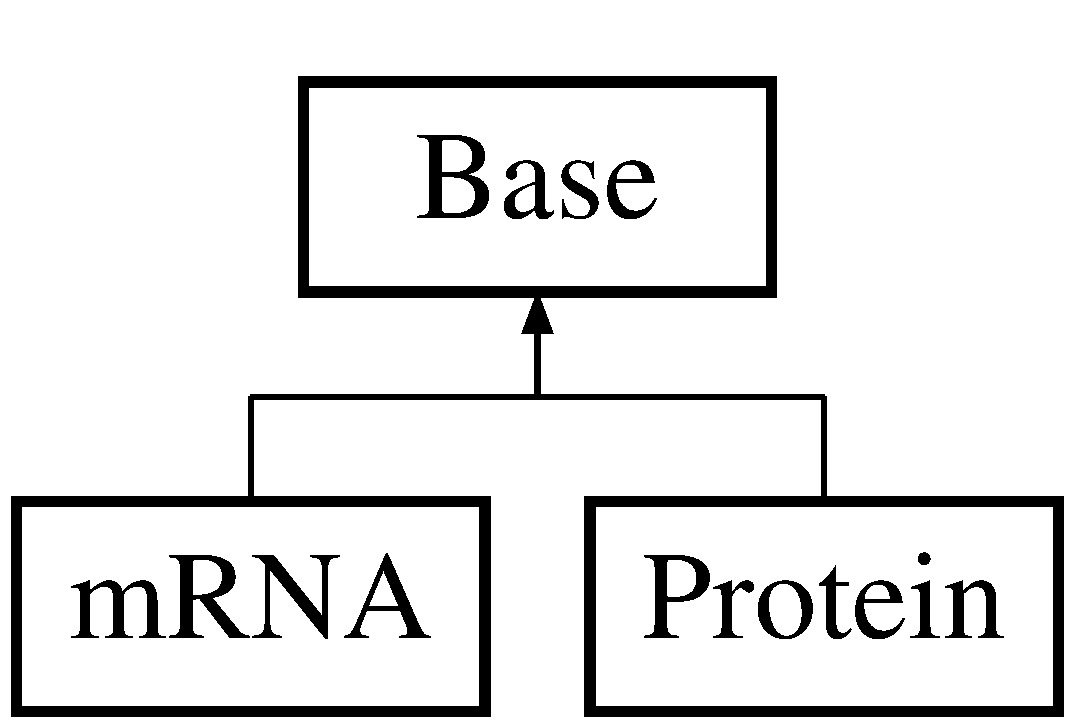
\includegraphics[height=2.000000cm]{class_base}
\end{center}
\end{figure}
\subsection*{Public Member Functions}
\begin{DoxyCompactItemize}
\item 
\hypertarget{class_base_a2539be60a003bf1153a87444870cfc50}{virtual void {\bfseries Compute} (int)=0}\label{class_base_a2539be60a003bf1153a87444870cfc50}

\end{DoxyCompactItemize}
\subsection*{Protected Attributes}
\begin{DoxyCompactItemize}
\item 
\hypertarget{class_base_af46b05bd03228ba15d40a05c15abffa0}{int {\bfseries id}}\label{class_base_af46b05bd03228ba15d40a05c15abffa0}

\item 
\hypertarget{class_base_afc939d650ee448e4b9e9302fdd8e6dae}{int {\bfseries length}}\label{class_base_afc939d650ee448e4b9e9302fdd8e6dae}

\item 
\hypertarget{class_base_a4c2c4261e4f2d0e7ebaf93bde00d3a26}{double {\bfseries dt}}\label{class_base_a4c2c4261e4f2d0e7ebaf93bde00d3a26}

\item 
\hypertarget{class_base_a262c09f4273320c819d77ec15a895980}{double $\ast$ {\bfseries abundance}}\label{class_base_a262c09f4273320c819d77ec15a895980}

\end{DoxyCompactItemize}
\subsection*{Friends}
\begin{DoxyCompactItemize}
\item 
\hypertarget{class_base_a50c933a62458087717ab7406e4cf01bc}{double $\ast$ {\bfseries Export} (int \&)}\label{class_base_a50c933a62458087717ab7406e4cf01bc}

\item 
\hypertarget{class_base_a868cf38fedb3c52291069b74bb198bf0}{void {\bfseries Simulate} ()}\label{class_base_a868cf38fedb3c52291069b74bb198bf0}

\end{DoxyCompactItemize}


The documentation for this class was generated from the following file\-:\begin{DoxyCompactItemize}
\item 
graph.\-h\end{DoxyCompactItemize}

\hypertarget{class_d_n_a}{\section{D\-N\-A Class Reference}
\label{class_d_n_a}\index{D\-N\-A@{D\-N\-A}}
}


{\ttfamily \#include $<$graph.\-h$>$}



Collaboration diagram for D\-N\-A\-:
\subsection*{Public Member Functions}
\begin{DoxyCompactItemize}
\item 
\hyperlink{class_d_n_a_a6d92499f10d383ac656e98694cc6c5e6}{D\-N\-A} (double, double, double)
\item 
void \hyperlink{class_d_n_a_a4db79a1d4530c15f30ec82cb8a502dda}{Connect} (\hyperlink{class_protein}{Protein} $\ast$)
\end{DoxyCompactItemize}
\subsection*{Private Attributes}
\begin{DoxyCompactItemize}
\item 
\hyperlink{class_protein}{Protein} $\ast$ \hyperlink{class_d_n_a_a08dd607e26ea53375e0c6d61c0c04ba9}{repressor}
\item 
double \hyperlink{class_d_n_a_ad9f4838495b5f66e494a8adb3384b919}{m}
\item 
double \hyperlink{class_d_n_a_a30c4d522f315530f9ce72e84afd6804c}{alpha}
\item 
double \hyperlink{class_d_n_a_a0dbd4309884cc23e9cbaf6cf4dc5ba0e}{epsilon}
\end{DoxyCompactItemize}
\subsection*{Friends}
\begin{DoxyCompactItemize}
\item 
class \hyperlink{class_d_n_a_a904bf77ec17baad950eb63ea5c40c6ea}{m\-R\-N\-A}
\end{DoxyCompactItemize}


\subsection{Constructor \& Destructor Documentation}
\hypertarget{class_d_n_a_a6d92499f10d383ac656e98694cc6c5e6}{\index{D\-N\-A@{D\-N\-A}!D\-N\-A@{D\-N\-A}}
\index{D\-N\-A@{D\-N\-A}!DNA@{D\-N\-A}}
\subsubsection[{D\-N\-A}]{\setlength{\rightskip}{0pt plus 5cm}D\-N\-A\-::\-D\-N\-A (
\begin{DoxyParamCaption}
\item[{double}]{mm, }
\item[{double}]{a, }
\item[{double}]{e}
\end{DoxyParamCaption}
)}}\label{class_d_n_a_a6d92499f10d383ac656e98694cc6c5e6}


\subsection{Member Function Documentation}
\hypertarget{class_d_n_a_a4db79a1d4530c15f30ec82cb8a502dda}{\index{D\-N\-A@{D\-N\-A}!Connect@{Connect}}
\index{Connect@{Connect}!DNA@{D\-N\-A}}
\subsubsection[{Connect}]{\setlength{\rightskip}{0pt plus 5cm}void D\-N\-A\-::\-Connect (
\begin{DoxyParamCaption}
\item[{{\bf Protein} $\ast$}]{p}
\end{DoxyParamCaption}
)}}\label{class_d_n_a_a4db79a1d4530c15f30ec82cb8a502dda}


\subsection{Friends And Related Function Documentation}
\hypertarget{class_d_n_a_a904bf77ec17baad950eb63ea5c40c6ea}{\index{D\-N\-A@{D\-N\-A}!m\-R\-N\-A@{m\-R\-N\-A}}
\index{m\-R\-N\-A@{m\-R\-N\-A}!DNA@{D\-N\-A}}
\subsubsection[{m\-R\-N\-A}]{\setlength{\rightskip}{0pt plus 5cm}friend class {\bf m\-R\-N\-A}\hspace{0.3cm}{\ttfamily [friend]}}}\label{class_d_n_a_a904bf77ec17baad950eb63ea5c40c6ea}


\subsection{Member Data Documentation}
\hypertarget{class_d_n_a_a30c4d522f315530f9ce72e84afd6804c}{\index{D\-N\-A@{D\-N\-A}!alpha@{alpha}}
\index{alpha@{alpha}!DNA@{D\-N\-A}}
\subsubsection[{alpha}]{\setlength{\rightskip}{0pt plus 5cm}double D\-N\-A\-::alpha\hspace{0.3cm}{\ttfamily [private]}}}\label{class_d_n_a_a30c4d522f315530f9ce72e84afd6804c}
\hypertarget{class_d_n_a_a0dbd4309884cc23e9cbaf6cf4dc5ba0e}{\index{D\-N\-A@{D\-N\-A}!epsilon@{epsilon}}
\index{epsilon@{epsilon}!DNA@{D\-N\-A}}
\subsubsection[{epsilon}]{\setlength{\rightskip}{0pt plus 5cm}double D\-N\-A\-::epsilon\hspace{0.3cm}{\ttfamily [private]}}}\label{class_d_n_a_a0dbd4309884cc23e9cbaf6cf4dc5ba0e}
\hypertarget{class_d_n_a_ad9f4838495b5f66e494a8adb3384b919}{\index{D\-N\-A@{D\-N\-A}!m@{m}}
\index{m@{m}!DNA@{D\-N\-A}}
\subsubsection[{m}]{\setlength{\rightskip}{0pt plus 5cm}double D\-N\-A\-::m\hspace{0.3cm}{\ttfamily [private]}}}\label{class_d_n_a_ad9f4838495b5f66e494a8adb3384b919}
\hypertarget{class_d_n_a_a08dd607e26ea53375e0c6d61c0c04ba9}{\index{D\-N\-A@{D\-N\-A}!repressor@{repressor}}
\index{repressor@{repressor}!DNA@{D\-N\-A}}
\subsubsection[{repressor}]{\setlength{\rightskip}{0pt plus 5cm}{\bf Protein}$\ast$ D\-N\-A\-::repressor\hspace{0.3cm}{\ttfamily [private]}}}\label{class_d_n_a_a08dd607e26ea53375e0c6d61c0c04ba9}


The documentation for this class was generated from the following file\-:\begin{DoxyCompactItemize}
\item 
\hyperlink{graph_8h}{graph.\-h}\end{DoxyCompactItemize}

\hypertarget{classweb_1_1_simulate___class_1_1_d_n_a___simulate}{\section{web.\-Simulate\-\_\-\-Class.\-D\-N\-A\-\_\-\-Simulate Class Reference}
\label{classweb_1_1_simulate___class_1_1_d_n_a___simulate}\index{web.\-Simulate\-\_\-\-Class.\-D\-N\-A\-\_\-\-Simulate@{web.\-Simulate\-\_\-\-Class.\-D\-N\-A\-\_\-\-Simulate}}
}


\subsubsection*{calculating \hyperlink{class_d_n_a}{D\-N\-A} simulation result } 


\subsection*{Public Member Functions}
\begin{DoxyCompactItemize}
\item 
def \hyperlink{classweb_1_1_simulate___class_1_1_d_n_a___simulate_a06ff5bd8c89a820405d937a5f8a837f3}{Set\-Data}
\begin{DoxyCompactList}\small\item\em Set data in class. \end{DoxyCompactList}\item 
def \hyperlink{classweb_1_1_simulate___class_1_1_d_n_a___simulate_ad17aed6fe820df86a76eae9e307c6fbc}{Set\-Activator}
\begin{DoxyCompactList}\small\item\em set activator in class \end{DoxyCompactList}\item 
def \hyperlink{classweb_1_1_simulate___class_1_1_d_n_a___simulate_af3ad470a356961ff4019e740f813e321}{Set\-Repressor}
\begin{DoxyCompactList}\small\item\em set repressor in class \end{DoxyCompactList}\item 
def \hyperlink{classweb_1_1_simulate___class_1_1_d_n_a___simulate_a467aabf0e04b68c0b813931ffdfbd86c}{Set\-Corepressor}
\begin{DoxyCompactList}\small\item\em set corepressor in class \end{DoxyCompactList}\item 
def \hyperlink{classweb_1_1_simulate___class_1_1_d_n_a___simulate_ad7ed3917ea1662b7d8ebded6ae6c9275}{Set\-Inducer}
\begin{DoxyCompactList}\small\item\em set inducer in class \end{DoxyCompactList}\end{DoxyCompactItemize}
\subsection*{Public Attributes}
\begin{DoxyCompactItemize}
\item 
\hypertarget{classweb_1_1_simulate___class_1_1_d_n_a___simulate_aa234468d2d8f7d04de55e93cb1ab0680}{{\bfseries Type}}\label{classweb_1_1_simulate___class_1_1_d_n_a___simulate_aa234468d2d8f7d04de55e93cb1ab0680}

\end{DoxyCompactItemize}
\subsection*{Static Public Attributes}
\begin{DoxyCompactItemize}
\item 
\hypertarget{classweb_1_1_simulate___class_1_1_d_n_a___simulate_a85da64f8805311e83467d99e2b4553a1}{string {\bfseries Type} = \char`\"{}\char`\"{}}\label{classweb_1_1_simulate___class_1_1_d_n_a___simulate_a85da64f8805311e83467d99e2b4553a1}

\item 
\hypertarget{classweb_1_1_simulate___class_1_1_d_n_a___simulate_a399330e85a7f32291f717b9eb846d080}{{\bfseries Copy\-Number} = None}\label{classweb_1_1_simulate___class_1_1_d_n_a___simulate_a399330e85a7f32291f717b9eb846d080}

\item 
\hypertarget{classweb_1_1_simulate___class_1_1_d_n_a___simulate_aea102d7a236466b4204e777bcbcfb1af}{{\bfseries T\-S\-Promoter} = None}\label{classweb_1_1_simulate___class_1_1_d_n_a___simulate_aea102d7a236466b4204e777bcbcfb1af}

\item 
\hypertarget{classweb_1_1_simulate___class_1_1_d_n_a___simulate_abc27d2561f40165607efd2b894fc18ef}{{\bfseries Leakage\-Rate} = None}\label{classweb_1_1_simulate___class_1_1_d_n_a___simulate_abc27d2561f40165607efd2b894fc18ef}

\item 
\hypertarget{classweb_1_1_simulate___class_1_1_d_n_a___simulate_af4973b509128336acfee906693d6af4b}{{\bfseries Ter\-E} = None}\label{classweb_1_1_simulate___class_1_1_d_n_a___simulate_af4973b509128336acfee906693d6af4b}

\item 
\hypertarget{classweb_1_1_simulate___class_1_1_d_n_a___simulate_ae298041c1b536e5ab369dff6cd3bac76}{{\bfseries Activator} = None}\label{classweb_1_1_simulate___class_1_1_d_n_a___simulate_ae298041c1b536e5ab369dff6cd3bac76}

\item 
\hypertarget{classweb_1_1_simulate___class_1_1_d_n_a___simulate_a6fc6961ca56a8c2f63f6289001092aa8}{{\bfseries Repressor} = None}\label{classweb_1_1_simulate___class_1_1_d_n_a___simulate_a6fc6961ca56a8c2f63f6289001092aa8}

\item 
\hypertarget{classweb_1_1_simulate___class_1_1_d_n_a___simulate_afe473f23d1ec1f5e576297bfa99b8d55}{{\bfseries Hill\-Coeff} = None}\label{classweb_1_1_simulate___class_1_1_d_n_a___simulate_afe473f23d1ec1f5e576297bfa99b8d55}

\item 
\hypertarget{classweb_1_1_simulate___class_1_1_d_n_a___simulate_ab41cef07d4729f53b81042b06b637fdf}{{\bfseries K} = None}\label{classweb_1_1_simulate___class_1_1_d_n_a___simulate_ab41cef07d4729f53b81042b06b637fdf}

\item 
\hypertarget{classweb_1_1_simulate___class_1_1_d_n_a___simulate_a4c01a78dc773cffe777a928a3ad8abcf}{{\bfseries Corep\-Const} = None}\label{classweb_1_1_simulate___class_1_1_d_n_a___simulate_a4c01a78dc773cffe777a928a3ad8abcf}

\item 
\hypertarget{classweb_1_1_simulate___class_1_1_d_n_a___simulate_a555c52a90c570dda2ccd7a0ec7eb00e2}{{\bfseries Ind\-Const} = None}\label{classweb_1_1_simulate___class_1_1_d_n_a___simulate_a555c52a90c570dda2ccd7a0ec7eb00e2}

\end{DoxyCompactItemize}


\subsection{Detailed Description}
\subsubsection*{calculating \hyperlink{class_d_n_a}{D\-N\-A} simulation result }

\subsection{Member Function Documentation}
\hypertarget{classweb_1_1_simulate___class_1_1_d_n_a___simulate_ad17aed6fe820df86a76eae9e307c6fbc}{\index{web\-::\-Simulate\-\_\-\-Class\-::\-D\-N\-A\-\_\-\-Simulate@{web\-::\-Simulate\-\_\-\-Class\-::\-D\-N\-A\-\_\-\-Simulate}!Set\-Activator@{Set\-Activator}}
\index{Set\-Activator@{Set\-Activator}!web::Simulate_Class::DNA_Simulate@{web\-::\-Simulate\-\_\-\-Class\-::\-D\-N\-A\-\_\-\-Simulate}}
\subsubsection[{Set\-Activator}]{\setlength{\rightskip}{0pt plus 5cm}def web.\-Simulate\-\_\-\-Class.\-D\-N\-A\-\_\-\-Simulate.\-Set\-Activator (
\begin{DoxyParamCaption}
\item[{}]{self, }
\item[{}]{activator, }
\item[{}]{k, }
\item[{}]{hillcoeff}
\end{DoxyParamCaption}
)}}\label{classweb_1_1_simulate___class_1_1_d_n_a___simulate_ad17aed6fe820df86a76eae9e307c6fbc}


set activator in class 


\begin{DoxyParams}{Parameters}
{\em activator} & name of activator \\
\hline
{\em k} & K value of activator \\
\hline
{\em hillcoeff} & hill coefficiency of activator\\
\hline
\end{DoxyParams}
\begin{DoxyReturn}{Returns}
return nothing 

 
\end{DoxyReturn}
\hypertarget{classweb_1_1_simulate___class_1_1_d_n_a___simulate_a467aabf0e04b68c0b813931ffdfbd86c}{\index{web\-::\-Simulate\-\_\-\-Class\-::\-D\-N\-A\-\_\-\-Simulate@{web\-::\-Simulate\-\_\-\-Class\-::\-D\-N\-A\-\_\-\-Simulate}!Set\-Corepressor@{Set\-Corepressor}}
\index{Set\-Corepressor@{Set\-Corepressor}!web::Simulate_Class::DNA_Simulate@{web\-::\-Simulate\-\_\-\-Class\-::\-D\-N\-A\-\_\-\-Simulate}}
\subsubsection[{Set\-Corepressor}]{\setlength{\rightskip}{0pt plus 5cm}def web.\-Simulate\-\_\-\-Class.\-D\-N\-A\-\_\-\-Simulate.\-Set\-Corepressor (
\begin{DoxyParamCaption}
\item[{}]{self, }
\item[{}]{corepressor, }
\item[{}]{k, }
\item[{}]{hillcoeff}
\end{DoxyParamCaption}
)}}\label{classweb_1_1_simulate___class_1_1_d_n_a___simulate_a467aabf0e04b68c0b813931ffdfbd86c}


set corepressor in class 


\begin{DoxyParams}{Parameters}
{\em corepressor} & name of corepressor \\
\hline
{\em k} & K value of corepressor \\
\hline
{\em hillcoeff} & hill coefficiency of corepressor\\
\hline
\end{DoxyParams}
\begin{DoxyReturn}{Returns}
return nothing 

 
\end{DoxyReturn}
\hypertarget{classweb_1_1_simulate___class_1_1_d_n_a___simulate_a06ff5bd8c89a820405d937a5f8a837f3}{\index{web\-::\-Simulate\-\_\-\-Class\-::\-D\-N\-A\-\_\-\-Simulate@{web\-::\-Simulate\-\_\-\-Class\-::\-D\-N\-A\-\_\-\-Simulate}!Set\-Data@{Set\-Data}}
\index{Set\-Data@{Set\-Data}!web::Simulate_Class::DNA_Simulate@{web\-::\-Simulate\-\_\-\-Class\-::\-D\-N\-A\-\_\-\-Simulate}}
\subsubsection[{Set\-Data}]{\setlength{\rightskip}{0pt plus 5cm}def web.\-Simulate\-\_\-\-Class.\-D\-N\-A\-\_\-\-Simulate.\-Set\-Data (
\begin{DoxyParamCaption}
\item[{}]{self, }
\item[{}]{ty, }
\item[{}]{copynumber, }
\item[{}]{tspromoter, }
\item[{}]{leakagerate, }
\item[{}]{tere}
\end{DoxyParamCaption}
)}}\label{classweb_1_1_simulate___class_1_1_d_n_a___simulate_a06ff5bd8c89a820405d937a5f8a837f3}


Set data in class. 


\begin{DoxyParams}{Parameters}
{\em ty} & type of data(constitutive, positive or negative) \\
\hline
{\em copynumber} & copy number of corresponding plasmid of component \\
\hline
{\em tspromoter} & T\-S\-Promoter of corresponding group of component \\
\hline
{\em leakagerate} & Leakage Rate of corresponding group of component \\
\hline
{\em tere} & terminator efficiency of corresponding group of component\\
\hline
\end{DoxyParams}
\begin{DoxyReturn}{Returns}
return nothing 

 
\end{DoxyReturn}
\hypertarget{classweb_1_1_simulate___class_1_1_d_n_a___simulate_ad7ed3917ea1662b7d8ebded6ae6c9275}{\index{web\-::\-Simulate\-\_\-\-Class\-::\-D\-N\-A\-\_\-\-Simulate@{web\-::\-Simulate\-\_\-\-Class\-::\-D\-N\-A\-\_\-\-Simulate}!Set\-Inducer@{Set\-Inducer}}
\index{Set\-Inducer@{Set\-Inducer}!web::Simulate_Class::DNA_Simulate@{web\-::\-Simulate\-\_\-\-Class\-::\-D\-N\-A\-\_\-\-Simulate}}
\subsubsection[{Set\-Inducer}]{\setlength{\rightskip}{0pt plus 5cm}def web.\-Simulate\-\_\-\-Class.\-D\-N\-A\-\_\-\-Simulate.\-Set\-Inducer (
\begin{DoxyParamCaption}
\item[{}]{self, }
\item[{}]{inducer, }
\item[{}]{k, }
\item[{}]{hillcoeff}
\end{DoxyParamCaption}
)}}\label{classweb_1_1_simulate___class_1_1_d_n_a___simulate_ad7ed3917ea1662b7d8ebded6ae6c9275}


set inducer in class 


\begin{DoxyParams}{Parameters}
{\em inducer} & name of inducer \\
\hline
{\em k} & K value of inducer \\
\hline
{\em hillcoeff} & hill coefficiency of inducer\\
\hline
\end{DoxyParams}
\begin{DoxyReturn}{Returns}
return nothing 

 
\end{DoxyReturn}
\hypertarget{classweb_1_1_simulate___class_1_1_d_n_a___simulate_af3ad470a356961ff4019e740f813e321}{\index{web\-::\-Simulate\-\_\-\-Class\-::\-D\-N\-A\-\_\-\-Simulate@{web\-::\-Simulate\-\_\-\-Class\-::\-D\-N\-A\-\_\-\-Simulate}!Set\-Repressor@{Set\-Repressor}}
\index{Set\-Repressor@{Set\-Repressor}!web::Simulate_Class::DNA_Simulate@{web\-::\-Simulate\-\_\-\-Class\-::\-D\-N\-A\-\_\-\-Simulate}}
\subsubsection[{Set\-Repressor}]{\setlength{\rightskip}{0pt plus 5cm}def web.\-Simulate\-\_\-\-Class.\-D\-N\-A\-\_\-\-Simulate.\-Set\-Repressor (
\begin{DoxyParamCaption}
\item[{}]{self, }
\item[{}]{repressor, }
\item[{}]{k, }
\item[{}]{hillcoeff}
\end{DoxyParamCaption}
)}}\label{classweb_1_1_simulate___class_1_1_d_n_a___simulate_af3ad470a356961ff4019e740f813e321}


set repressor in class 


\begin{DoxyParams}{Parameters}
{\em repressor} & name of repressor \\
\hline
{\em k} & K value of repressor \\
\hline
{\em hillcoeff} & hill coefficiency of repressor\\
\hline
\end{DoxyParams}
\begin{DoxyReturn}{Returns}
return nothing 

 
\end{DoxyReturn}


The documentation for this class was generated from the following file\-:\begin{DoxyCompactItemize}
\item 
\hyperlink{_simulate___class_8py}{Simulate\-\_\-\-Class.\-py}\end{DoxyCompactItemize}

\hypertarget{classweb_1_1encrypt_1_1_encrypt}{\section{web.\-encrypt.\-Encrypt Class Reference}
\label{classweb_1_1encrypt_1_1_encrypt}\index{web.\-encrypt.\-Encrypt@{web.\-encrypt.\-Encrypt}}
}


\subsubsection*{the class that can provide R\-S\-A method } 


\subsection*{Public Member Functions}
\begin{DoxyCompactItemize}
\item 
def \hyperlink{classweb_1_1encrypt_1_1_encrypt_a7ac013ef450d16011e76b7af95c25f3d}{\-\_\-\-\_\-init\-\_\-\-\_\-}
\item 
def \hyperlink{classweb_1_1encrypt_1_1_encrypt_ad9c50ce7eec9117081e4d86a9bfd87c9}{get\-Public\-Key}
\begin{DoxyCompactList}\small\item\em get the public key \end{DoxyCompactList}\item 
def \hyperlink{classweb_1_1encrypt_1_1_encrypt_afcab4d2eea9fe8213086a46253e72316}{decrypt}
\begin{DoxyCompactList}\small\item\em decrypt a string \end{DoxyCompactList}\end{DoxyCompactItemize}
\subsection*{Public Attributes}
\begin{DoxyCompactItemize}
\item 
\hyperlink{classweb_1_1encrypt_1_1_encrypt_a1e54531b2aac210260199608edc7f62c}{public\-Key}
\item 
\hyperlink{classweb_1_1encrypt_1_1_encrypt_a1145a5b40bf2a2ff38383b34d4d86dc8}{private\-Key}
\end{DoxyCompactItemize}


\subsection{Detailed Description}
\subsubsection*{the class that can provide R\-S\-A method }

\subsection{Constructor \& Destructor Documentation}
\hypertarget{classweb_1_1encrypt_1_1_encrypt_a7ac013ef450d16011e76b7af95c25f3d}{\index{web\-::encrypt\-::\-Encrypt@{web\-::encrypt\-::\-Encrypt}!\-\_\-\-\_\-init\-\_\-\-\_\-@{\-\_\-\-\_\-init\-\_\-\-\_\-}}
\index{\-\_\-\-\_\-init\-\_\-\-\_\-@{\-\_\-\-\_\-init\-\_\-\-\_\-}!web::encrypt::Encrypt@{web\-::encrypt\-::\-Encrypt}}
\subsubsection[{\-\_\-\-\_\-init\-\_\-\-\_\-}]{\setlength{\rightskip}{0pt plus 5cm}def web.\-encrypt.\-Encrypt.\-\_\-\-\_\-init\-\_\-\-\_\- (
\begin{DoxyParamCaption}
\item[{}]{self}
\end{DoxyParamCaption}
)}}\label{classweb_1_1encrypt_1_1_encrypt_a7ac013ef450d16011e76b7af95c25f3d}


\subsection{Member Function Documentation}
\hypertarget{classweb_1_1encrypt_1_1_encrypt_afcab4d2eea9fe8213086a46253e72316}{\index{web\-::encrypt\-::\-Encrypt@{web\-::encrypt\-::\-Encrypt}!decrypt@{decrypt}}
\index{decrypt@{decrypt}!web::encrypt::Encrypt@{web\-::encrypt\-::\-Encrypt}}
\subsubsection[{decrypt}]{\setlength{\rightskip}{0pt plus 5cm}def web.\-encrypt.\-Encrypt.\-decrypt (
\begin{DoxyParamCaption}
\item[{}]{self, }
\item[{}]{crypto}
\end{DoxyParamCaption}
)}}\label{classweb_1_1encrypt_1_1_encrypt_afcab4d2eea9fe8213086a46253e72316}


decrypt a string 


\begin{DoxyParams}{Parameters}
{\em self} & \\
\hline
{\em crypto} & the crypto string\\
\hline
\end{DoxyParams}
\begin{DoxyReturn}{Returns}
return the original string using the private\-Key 

 
\end{DoxyReturn}
\hypertarget{classweb_1_1encrypt_1_1_encrypt_ad9c50ce7eec9117081e4d86a9bfd87c9}{\index{web\-::encrypt\-::\-Encrypt@{web\-::encrypt\-::\-Encrypt}!get\-Public\-Key@{get\-Public\-Key}}
\index{get\-Public\-Key@{get\-Public\-Key}!web::encrypt::Encrypt@{web\-::encrypt\-::\-Encrypt}}
\subsubsection[{get\-Public\-Key}]{\setlength{\rightskip}{0pt plus 5cm}def web.\-encrypt.\-Encrypt.\-get\-Public\-Key (
\begin{DoxyParamCaption}
\item[{}]{self}
\end{DoxyParamCaption}
)}}\label{classweb_1_1encrypt_1_1_encrypt_ad9c50ce7eec9117081e4d86a9bfd87c9}


get the public key 


\begin{DoxyParams}{Parameters}
{\em self} & \\
\hline
\end{DoxyParams}
\begin{DoxyReturn}{Returns}
return the public key 

 
\end{DoxyReturn}


\subsection{Member Data Documentation}
\hypertarget{classweb_1_1encrypt_1_1_encrypt_a1145a5b40bf2a2ff38383b34d4d86dc8}{\index{web\-::encrypt\-::\-Encrypt@{web\-::encrypt\-::\-Encrypt}!private\-Key@{private\-Key}}
\index{private\-Key@{private\-Key}!web::encrypt::Encrypt@{web\-::encrypt\-::\-Encrypt}}
\subsubsection[{private\-Key}]{\setlength{\rightskip}{0pt plus 5cm}web.\-encrypt.\-Encrypt.\-private\-Key}}\label{classweb_1_1encrypt_1_1_encrypt_a1145a5b40bf2a2ff38383b34d4d86dc8}
\hypertarget{classweb_1_1encrypt_1_1_encrypt_a1e54531b2aac210260199608edc7f62c}{\index{web\-::encrypt\-::\-Encrypt@{web\-::encrypt\-::\-Encrypt}!public\-Key@{public\-Key}}
\index{public\-Key@{public\-Key}!web::encrypt::Encrypt@{web\-::encrypt\-::\-Encrypt}}
\subsubsection[{public\-Key}]{\setlength{\rightskip}{0pt plus 5cm}web.\-encrypt.\-Encrypt.\-public\-Key}}\label{classweb_1_1encrypt_1_1_encrypt_a1e54531b2aac210260199608edc7f62c}


The documentation for this class was generated from the following file\-:\begin{DoxyCompactItemize}
\item 
\hyperlink{encrypt_8py}{encrypt.\-py}\end{DoxyCompactItemize}

\hypertarget{classweb_1_1_simulate___class_1_1_illegal_setting}{\section{web.\-Simulate\-\_\-\-Class.\-Illegal\-Setting Class Reference}
\label{classweb_1_1_simulate___class_1_1_illegal_setting}\index{web.\-Simulate\-\_\-\-Class.\-Illegal\-Setting@{web.\-Simulate\-\_\-\-Class.\-Illegal\-Setting}}
}
Inheritance diagram for web.\-Simulate\-\_\-\-Class.\-Illegal\-Setting\-:\begin{figure}[H]
\begin{center}
\leavevmode
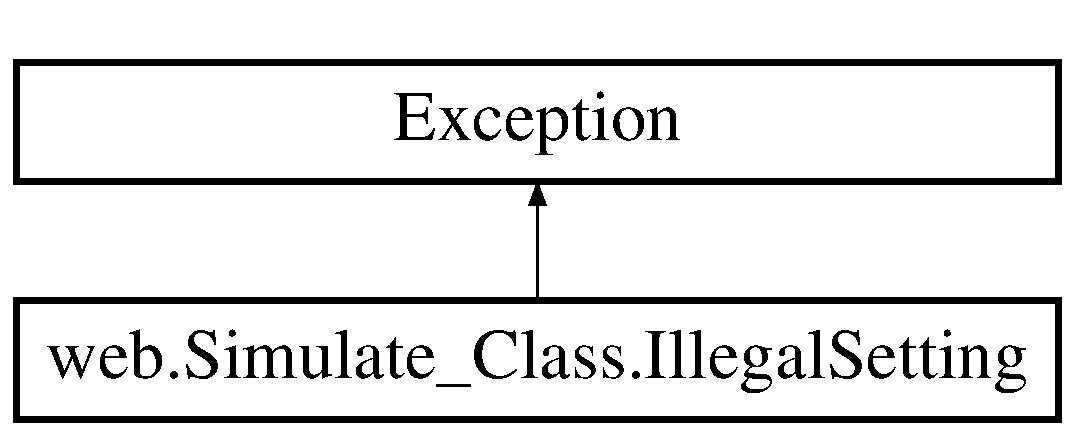
\includegraphics[height=2.000000cm]{classweb_1_1_simulate___class_1_1_illegal_setting}
\end{center}
\end{figure}


The documentation for this class was generated from the following file\-:\begin{DoxyCompactItemize}
\item 
\hyperlink{_simulate___class_8py}{Simulate\-\_\-\-Class.\-py}\end{DoxyCompactItemize}

\hypertarget{classweb_1_1_simulate___class_1_1_invalid_parameter}{\section{web.\-Simulate\-\_\-\-Class.\-Invalid\-Parameter Class Reference}
\label{classweb_1_1_simulate___class_1_1_invalid_parameter}\index{web.\-Simulate\-\_\-\-Class.\-Invalid\-Parameter@{web.\-Simulate\-\_\-\-Class.\-Invalid\-Parameter}}
}
Inheritance diagram for web.\-Simulate\-\_\-\-Class.\-Invalid\-Parameter\-:\begin{figure}[H]
\begin{center}
\leavevmode
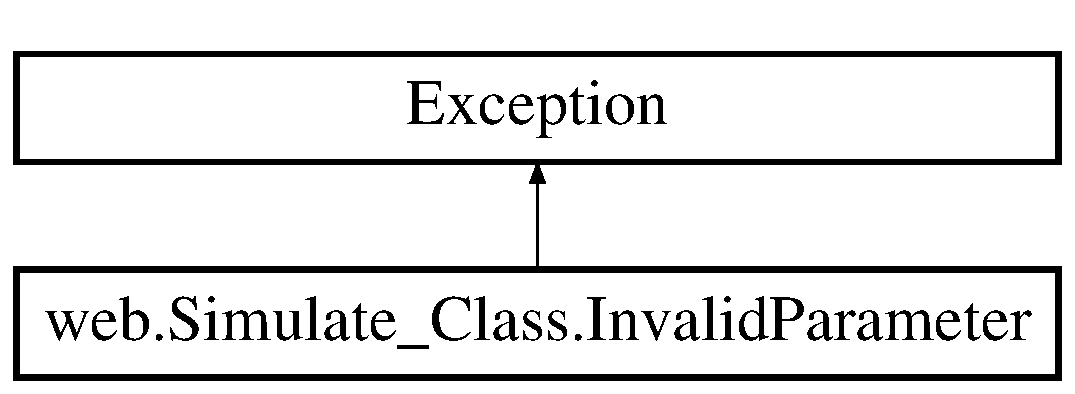
\includegraphics[height=2.000000cm]{classweb_1_1_simulate___class_1_1_invalid_parameter}
\end{center}
\end{figure}


The documentation for this class was generated from the following file\-:\begin{DoxyCompactItemize}
\item 
\hyperlink{_simulate___class_8py}{Simulate\-\_\-\-Class.\-py}\end{DoxyCompactItemize}

\hypertarget{classweb_1_1modeling_1_1modeling}{\section{web.\-modeling.\-modeling Class Reference}
\label{classweb_1_1modeling_1_1modeling}\index{web.\-modeling.\-modeling@{web.\-modeling.\-modeling}}
}
\subsection*{Public Member Functions}
\begin{DoxyCompactItemize}
\item 
\hypertarget{classweb_1_1modeling_1_1modeling_a7898b83d4325000468bf3b19dd0cf009}{def {\bfseries \-\_\-\-\_\-init\-\_\-\-\_\-}}\label{classweb_1_1modeling_1_1modeling_a7898b83d4325000468bf3b19dd0cf009}

\item 
\hypertarget{classweb_1_1modeling_1_1modeling_ad21a9030cd229dc73b6318abff8733e6}{def {\bfseries depressing\-Function}}\label{classweb_1_1modeling_1_1modeling_ad21a9030cd229dc73b6318abff8733e6}

\end{DoxyCompactItemize}
\subsection*{Public Attributes}
\begin{DoxyCompactItemize}
\item 
\hypertarget{classweb_1_1modeling_1_1modeling_affbc9a007f7b35ef14afce145c58bf18}{{\bfseries db}}\label{classweb_1_1modeling_1_1modeling_affbc9a007f7b35ef14afce145c58bf18}

\item 
\hypertarget{classweb_1_1modeling_1_1modeling_a7305302d2cd99859e0641132ac9ac0f3}{{\bfseries A\-Expression\-Value\-Record}}\label{classweb_1_1modeling_1_1modeling_a7305302d2cd99859e0641132ac9ac0f3}

\item 
\hypertarget{classweb_1_1modeling_1_1modeling_a8fb8abde81146a93ee8f7e0ec8fedf7f}{{\bfseries A\-Promoter}}\label{classweb_1_1modeling_1_1modeling_a8fb8abde81146a93ee8f7e0ec8fedf7f}

\item 
\hypertarget{classweb_1_1modeling_1_1modeling_ad8689aeec5372b03c7455f53d32cc1d8}{{\bfseries A\-Plasmid\-Backbone}}\label{classweb_1_1modeling_1_1modeling_ad8689aeec5372b03c7455f53d32cc1d8}

\item 
\hypertarget{classweb_1_1modeling_1_1modeling_ab2ab0f6fc77ef28f58988fffed95fa74}{{\bfseries B\-Expression\-Value\-Record}}\label{classweb_1_1modeling_1_1modeling_ab2ab0f6fc77ef28f58988fffed95fa74}

\item 
\hypertarget{classweb_1_1modeling_1_1modeling_a96fa7c50494910911cd1bb5e0fd6c247}{{\bfseries B\-Promoter}}\label{classweb_1_1modeling_1_1modeling_a96fa7c50494910911cd1bb5e0fd6c247}

\item 
\hypertarget{classweb_1_1modeling_1_1modeling_a18419f401d8b614ce048cd4f61fe3720}{{\bfseries B\-Plasmid\-Backbone}}\label{classweb_1_1modeling_1_1modeling_a18419f401d8b614ce048cd4f61fe3720}

\item 
\hypertarget{classweb_1_1modeling_1_1modeling_a6da71e7f269b891b00412fc6897c9747}{{\bfseries Protein\-A}}\label{classweb_1_1modeling_1_1modeling_a6da71e7f269b891b00412fc6897c9747}

\item 
\hypertarget{classweb_1_1modeling_1_1modeling_aff3389950cb599a298b6370a2dad0185}{{\bfseries Protein\-B}}\label{classweb_1_1modeling_1_1modeling_aff3389950cb599a298b6370a2dad0185}

\item 
\hypertarget{classweb_1_1modeling_1_1modeling_a4cc11ff2adba839163240e9ea66ef398}{{\bfseries R\-B\-S}}\label{classweb_1_1modeling_1_1modeling_a4cc11ff2adba839163240e9ea66ef398}

\item 
\hypertarget{classweb_1_1modeling_1_1modeling_a0314c62c089feb8e1d85448cc94f7900}{{\bfseries Repressor\-Table}}\label{classweb_1_1modeling_1_1modeling_a0314c62c089feb8e1d85448cc94f7900}

\end{DoxyCompactItemize}


The documentation for this class was generated from the following file\-:\begin{DoxyCompactItemize}
\item 
modeling.\-py\end{DoxyCompactItemize}

\hypertarget{classm_r_n_a}{\section{m\-R\-N\-A Class Reference}
\label{classm_r_n_a}\index{m\-R\-N\-A@{m\-R\-N\-A}}
}


{\ttfamily \#include $<$graph.\-h$>$}

Inheritance diagram for m\-R\-N\-A\-:\begin{figure}[H]
\begin{center}
\leavevmode
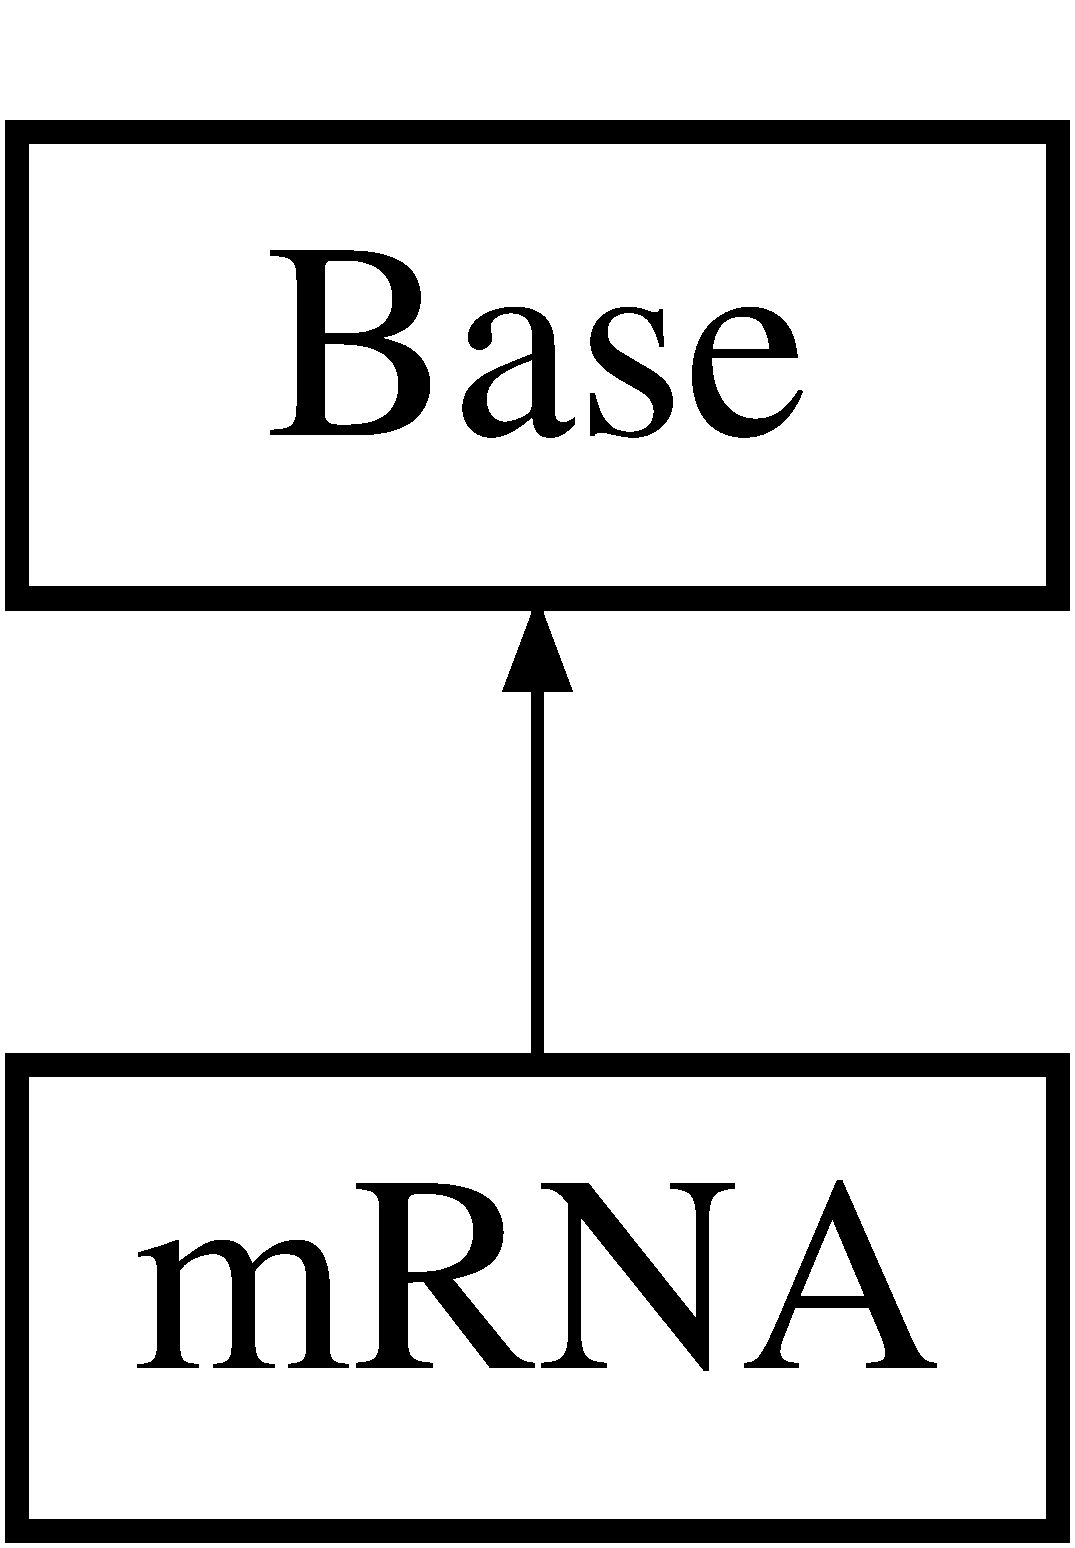
\includegraphics[height=2.000000cm]{classm_r_n_a}
\end{center}
\end{figure}
\subsection*{Public Member Functions}
\begin{DoxyCompactItemize}
\item 
\hyperlink{classm_r_n_a_a1fc26dc1fe542e23f9d374533600b9fb}{m\-R\-N\-A} (double, double, double, double)
\item 
void \hyperlink{classm_r_n_a_ac010324e6b1dc61fb8e1391b219acb2c}{Connect} (\hyperlink{class_d_n_a}{D\-N\-A} $\ast$)
\item 
void \hyperlink{classm_r_n_a_a490f8026d612c405ce2678a4d15cf7a8}{Compute} (int)
\end{DoxyCompactItemize}
\subsection*{Private Attributes}
\begin{DoxyCompactItemize}
\item 
\hyperlink{class_d_n_a}{D\-N\-A} $\ast$ \hyperlink{classm_r_n_a_ace67bd5431ec023732e05049e5ca9a4b}{dna}
\item 
double \hyperlink{classm_r_n_a_a07cdcbe61a2af4fc74751521e0c7920e}{v\-\_\-max}
\item 
double \hyperlink{classm_r_n_a_ace3b5460f5ed647cbe52e6a86e8d6ef7}{k\-\_\-mich}
\item 
double \hyperlink{classm_r_n_a_ac4e84c4700ca924196809e36fa17c5b7}{k\-\_\-deg}
\end{DoxyCompactItemize}
\subsection*{Friends}
\begin{DoxyCompactItemize}
\item 
class \hyperlink{classm_r_n_a_a2cc8b86817f46f61585ecf591984f8eb}{Protein}
\end{DoxyCompactItemize}
\subsection*{Additional Inherited Members}


\subsection{Constructor \& Destructor Documentation}
\hypertarget{classm_r_n_a_a1fc26dc1fe542e23f9d374533600b9fb}{\index{m\-R\-N\-A@{m\-R\-N\-A}!m\-R\-N\-A@{m\-R\-N\-A}}
\index{m\-R\-N\-A@{m\-R\-N\-A}!mRNA@{m\-R\-N\-A}}
\subsubsection[{m\-R\-N\-A}]{\setlength{\rightskip}{0pt plus 5cm}m\-R\-N\-A\-::m\-R\-N\-A (
\begin{DoxyParamCaption}
\item[{double}]{v, }
\item[{double}]{km, }
\item[{double}]{kd, }
\item[{double}]{ini}
\end{DoxyParamCaption}
)}}\label{classm_r_n_a_a1fc26dc1fe542e23f9d374533600b9fb}


\subsection{Member Function Documentation}
\hypertarget{classm_r_n_a_a490f8026d612c405ce2678a4d15cf7a8}{\index{m\-R\-N\-A@{m\-R\-N\-A}!Compute@{Compute}}
\index{Compute@{Compute}!mRNA@{m\-R\-N\-A}}
\subsubsection[{Compute}]{\setlength{\rightskip}{0pt plus 5cm}void m\-R\-N\-A\-::\-Compute (
\begin{DoxyParamCaption}
\item[{int}]{n}
\end{DoxyParamCaption}
)\hspace{0.3cm}{\ttfamily [virtual]}}}\label{classm_r_n_a_a490f8026d612c405ce2678a4d15cf7a8}


Implements \hyperlink{class_base_a2539be60a003bf1153a87444870cfc50}{Base}.

\hypertarget{classm_r_n_a_ac010324e6b1dc61fb8e1391b219acb2c}{\index{m\-R\-N\-A@{m\-R\-N\-A}!Connect@{Connect}}
\index{Connect@{Connect}!mRNA@{m\-R\-N\-A}}
\subsubsection[{Connect}]{\setlength{\rightskip}{0pt plus 5cm}void m\-R\-N\-A\-::\-Connect (
\begin{DoxyParamCaption}
\item[{{\bf D\-N\-A} $\ast$}]{d}
\end{DoxyParamCaption}
)}}\label{classm_r_n_a_ac010324e6b1dc61fb8e1391b219acb2c}


\subsection{Friends And Related Function Documentation}
\hypertarget{classm_r_n_a_a2cc8b86817f46f61585ecf591984f8eb}{\index{m\-R\-N\-A@{m\-R\-N\-A}!Protein@{Protein}}
\index{Protein@{Protein}!mRNA@{m\-R\-N\-A}}
\subsubsection[{Protein}]{\setlength{\rightskip}{0pt plus 5cm}friend class {\bf Protein}\hspace{0.3cm}{\ttfamily [friend]}}}\label{classm_r_n_a_a2cc8b86817f46f61585ecf591984f8eb}


\subsection{Member Data Documentation}
\hypertarget{classm_r_n_a_ace67bd5431ec023732e05049e5ca9a4b}{\index{m\-R\-N\-A@{m\-R\-N\-A}!dna@{dna}}
\index{dna@{dna}!mRNA@{m\-R\-N\-A}}
\subsubsection[{dna}]{\setlength{\rightskip}{0pt plus 5cm}{\bf D\-N\-A}$\ast$ m\-R\-N\-A\-::dna\hspace{0.3cm}{\ttfamily [private]}}}\label{classm_r_n_a_ace67bd5431ec023732e05049e5ca9a4b}
\hypertarget{classm_r_n_a_ac4e84c4700ca924196809e36fa17c5b7}{\index{m\-R\-N\-A@{m\-R\-N\-A}!k\-\_\-deg@{k\-\_\-deg}}
\index{k\-\_\-deg@{k\-\_\-deg}!mRNA@{m\-R\-N\-A}}
\subsubsection[{k\-\_\-deg}]{\setlength{\rightskip}{0pt plus 5cm}double m\-R\-N\-A\-::k\-\_\-deg\hspace{0.3cm}{\ttfamily [private]}}}\label{classm_r_n_a_ac4e84c4700ca924196809e36fa17c5b7}
\hypertarget{classm_r_n_a_ace3b5460f5ed647cbe52e6a86e8d6ef7}{\index{m\-R\-N\-A@{m\-R\-N\-A}!k\-\_\-mich@{k\-\_\-mich}}
\index{k\-\_\-mich@{k\-\_\-mich}!mRNA@{m\-R\-N\-A}}
\subsubsection[{k\-\_\-mich}]{\setlength{\rightskip}{0pt plus 5cm}double m\-R\-N\-A\-::k\-\_\-mich\hspace{0.3cm}{\ttfamily [private]}}}\label{classm_r_n_a_ace3b5460f5ed647cbe52e6a86e8d6ef7}
\hypertarget{classm_r_n_a_a07cdcbe61a2af4fc74751521e0c7920e}{\index{m\-R\-N\-A@{m\-R\-N\-A}!v\-\_\-max@{v\-\_\-max}}
\index{v\-\_\-max@{v\-\_\-max}!mRNA@{m\-R\-N\-A}}
\subsubsection[{v\-\_\-max}]{\setlength{\rightskip}{0pt plus 5cm}double m\-R\-N\-A\-::v\-\_\-max\hspace{0.3cm}{\ttfamily [private]}}}\label{classm_r_n_a_a07cdcbe61a2af4fc74751521e0c7920e}


The documentation for this class was generated from the following file\-:\begin{DoxyCompactItemize}
\item 
\hyperlink{graph_8h}{graph.\-h}\end{DoxyCompactItemize}

\hypertarget{classweb_1_1_simulate___class_1_1m_r_n_a___simulate}{\section{web.\-Simulate\-\_\-\-Class.\-m\-R\-N\-A\-\_\-\-Simulate Class Reference}
\label{classweb_1_1_simulate___class_1_1m_r_n_a___simulate}\index{web.\-Simulate\-\_\-\-Class.\-m\-R\-N\-A\-\_\-\-Simulate@{web.\-Simulate\-\_\-\-Class.\-m\-R\-N\-A\-\_\-\-Simulate}}
}
\subsection*{Public Member Functions}
\begin{DoxyCompactItemize}
\item 
\hypertarget{classweb_1_1_simulate___class_1_1m_r_n_a___simulate_aafa306e52e6cd8565e2abc96336bacbf}{def {\bfseries Set\-Data}}\label{classweb_1_1_simulate___class_1_1m_r_n_a___simulate_aafa306e52e6cd8565e2abc96336bacbf}

\item 
\hypertarget{classweb_1_1_simulate___class_1_1m_r_n_a___simulate_a4af7cedb8c3df5fcd581affc57e7afca}{def {\bfseries Connect}}\label{classweb_1_1_simulate___class_1_1m_r_n_a___simulate_a4af7cedb8c3df5fcd581affc57e7afca}

\item 
\hypertarget{classweb_1_1_simulate___class_1_1m_r_n_a___simulate_a8b9036fb94041c3247f18ab5b7d28216}{def {\bfseries Ini\-Concen}}\label{classweb_1_1_simulate___class_1_1m_r_n_a___simulate_a8b9036fb94041c3247f18ab5b7d28216}

\item 
\hypertarget{classweb_1_1_simulate___class_1_1m_r_n_a___simulate_ab96aa173aa7a27b60a60c3cddc05b41b}{def {\bfseries Compute\-\_\-\-Concen}}\label{classweb_1_1_simulate___class_1_1m_r_n_a___simulate_ab96aa173aa7a27b60a60c3cddc05b41b}

\end{DoxyCompactItemize}
\subsection*{Public Attributes}
\begin{DoxyCompactItemize}
\item 
\hypertarget{classweb_1_1_simulate___class_1_1m_r_n_a___simulate_a89a68a9662a7c802b3b9d7436649920f}{{\bfseries Concen}}\label{classweb_1_1_simulate___class_1_1m_r_n_a___simulate_a89a68a9662a7c802b3b9d7436649920f}

\end{DoxyCompactItemize}
\subsection*{Static Public Attributes}
\begin{DoxyCompactItemize}
\item 
\hypertarget{classweb_1_1_simulate___class_1_1m_r_n_a___simulate_aff71f631c32c2e13789fb4f2e413feb5}{{\bfseries Dt} = None}\label{classweb_1_1_simulate___class_1_1m_r_n_a___simulate_aff71f631c32c2e13789fb4f2e413feb5}

\item 
\hypertarget{classweb_1_1_simulate___class_1_1m_r_n_a___simulate_a1fbca90fe65ec4c5a6e07ef6aab4ef4f}{{\bfseries Time\-Len} = None}\label{classweb_1_1_simulate___class_1_1m_r_n_a___simulate_a1fbca90fe65ec4c5a6e07ef6aab4ef4f}

\item 
\hypertarget{classweb_1_1_simulate___class_1_1m_r_n_a___simulate_a8d08b83d4273c7c21c20fedc33d71d46}{list {\bfseries Concen} = \mbox{[}$\,$\mbox{]}}\label{classweb_1_1_simulate___class_1_1m_r_n_a___simulate_a8d08b83d4273c7c21c20fedc33d71d46}

\item 
\hypertarget{classweb_1_1_simulate___class_1_1m_r_n_a___simulate_a93f85081905b6beb3c395793f15b2956}{{\bfseries D\-N\-A} = None}\label{classweb_1_1_simulate___class_1_1m_r_n_a___simulate_a93f85081905b6beb3c395793f15b2956}

\item 
\hypertarget{classweb_1_1_simulate___class_1_1m_r_n_a___simulate_a0f1d34dcecf981a5dac457ce57260ead}{{\bfseries Transl\-E} = None}\label{classweb_1_1_simulate___class_1_1m_r_n_a___simulate_a0f1d34dcecf981a5dac457ce57260ead}

\item 
\hypertarget{classweb_1_1_simulate___class_1_1m_r_n_a___simulate_ab0f22fbf0ee72dcac2743805b982aab8}{{\bfseries Deg\-Rate} = None}\label{classweb_1_1_simulate___class_1_1m_r_n_a___simulate_ab0f22fbf0ee72dcac2743805b982aab8}

\end{DoxyCompactItemize}


The documentation for this class was generated from the following file\-:\begin{DoxyCompactItemize}
\item 
\hyperlink{_simulate___class_8py}{Simulate\-\_\-\-Class.\-py}\end{DoxyCompactItemize}

\hypertarget{class_protein}{\section{Protein Class Reference}
\label{class_protein}\index{Protein@{Protein}}
}
Inheritance diagram for Protein\-:\begin{figure}[H]
\begin{center}
\leavevmode
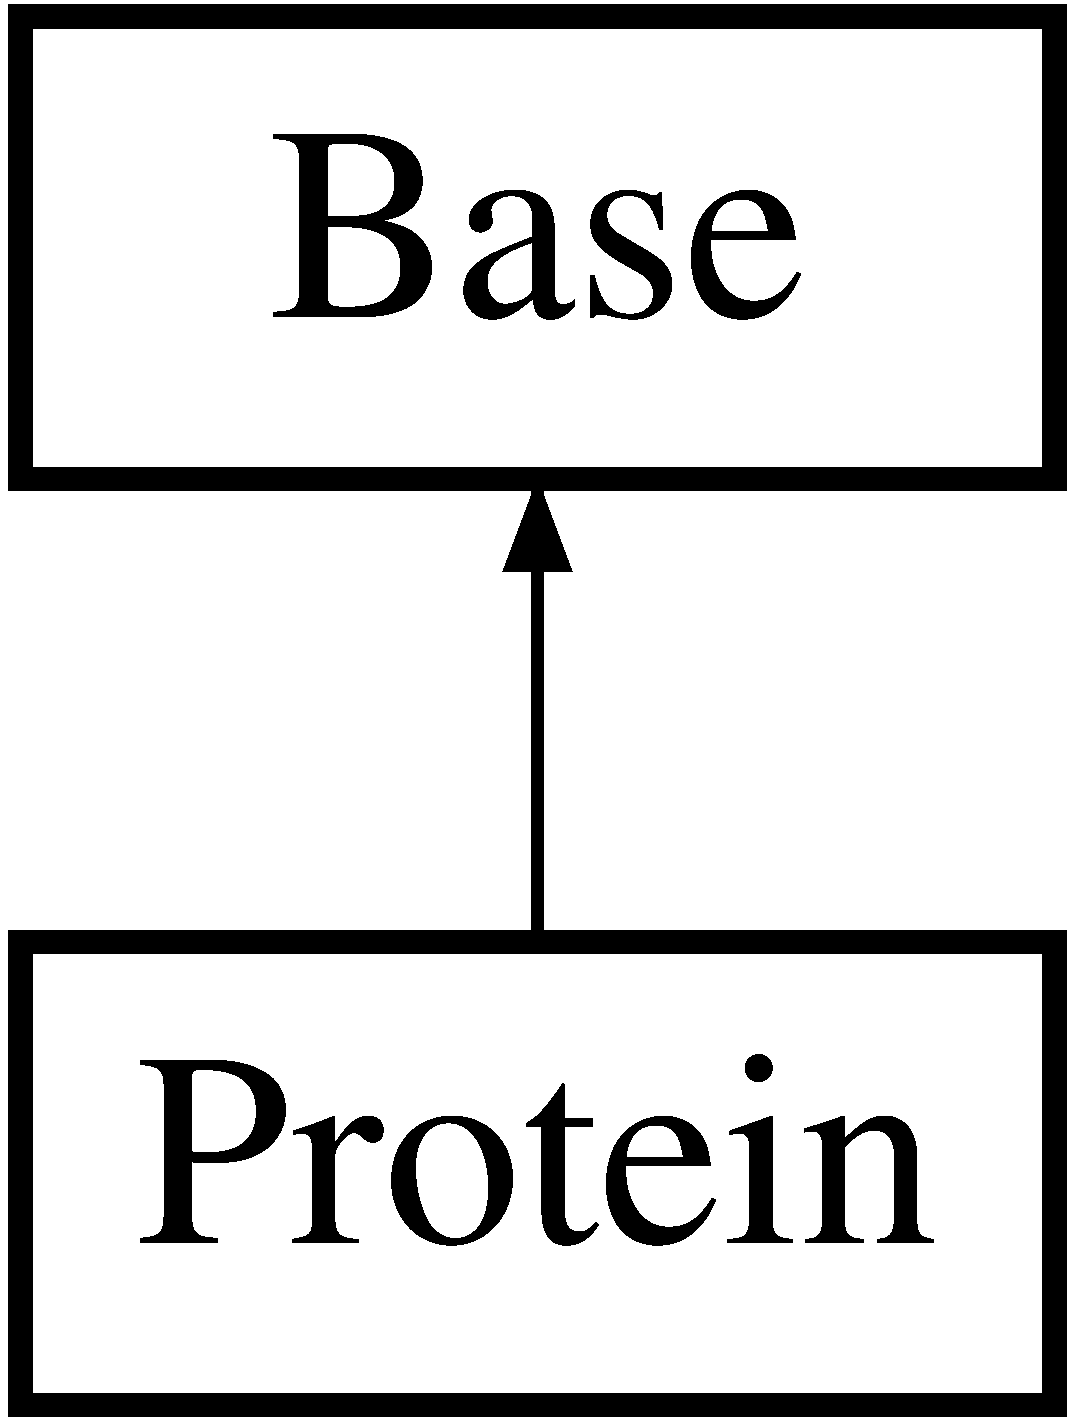
\includegraphics[height=2.000000cm]{class_protein}
\end{center}
\end{figure}
\subsection*{Public Member Functions}
\begin{DoxyCompactItemize}
\item 
\hypertarget{class_protein_a9f0a706232fd3e68c15263e2102fec02}{{\bfseries Protein} (double, double)}\label{class_protein_a9f0a706232fd3e68c15263e2102fec02}

\item 
\hypertarget{class_protein_a52cf8da9e08eeb67b44114af2d12f45c}{void {\bfseries Connect} (\hyperlink{classm_r_n_a}{m\-R\-N\-A} $\ast$)}\label{class_protein_a52cf8da9e08eeb67b44114af2d12f45c}

\item 
\hypertarget{class_protein_af977204f0e2ffe5544bcab971d5eeb0d}{void {\bfseries Compute} (int)}\label{class_protein_af977204f0e2ffe5544bcab971d5eeb0d}

\end{DoxyCompactItemize}
\subsection*{Friends}
\begin{DoxyCompactItemize}
\item 
\hypertarget{class_protein_a904bf77ec17baad950eb63ea5c40c6ea}{class {\bfseries m\-R\-N\-A}}\label{class_protein_a904bf77ec17baad950eb63ea5c40c6ea}

\end{DoxyCompactItemize}
\subsection*{Additional Inherited Members}


The documentation for this class was generated from the following file\-:\begin{DoxyCompactItemize}
\item 
graph.\-h\end{DoxyCompactItemize}

\hypertarget{classweb_1_1_simulate___class_1_1_protein___simulate}{\section{web.\-Simulate\-\_\-\-Class.\-Protein\-\_\-\-Simulate Class Reference}
\label{classweb_1_1_simulate___class_1_1_protein___simulate}\index{web.\-Simulate\-\_\-\-Class.\-Protein\-\_\-\-Simulate@{web.\-Simulate\-\_\-\-Class.\-Protein\-\_\-\-Simulate}}
}
\subsection*{Public Member Functions}
\begin{DoxyCompactItemize}
\item 
def \hyperlink{classweb_1_1_simulate___class_1_1_protein___simulate_aed90abad02aad5dc6ac31a344032b8c8}{Set\-Data}
\item 
def \hyperlink{classweb_1_1_simulate___class_1_1_protein___simulate_a25ef40b09e3b2ad608d7fd32dfbbc552}{Ini\-Concen}
\item 
def \hyperlink{classweb_1_1_simulate___class_1_1_protein___simulate_ad8e95c5ff42680746fd7f0e66dfefa95}{Connect}
\item 
def \hyperlink{classweb_1_1_simulate___class_1_1_protein___simulate_ac7de7384d587c3bc575e762ad40d8446}{Compute\-\_\-\-Concen}
\end{DoxyCompactItemize}
\subsection*{Public Attributes}
\begin{DoxyCompactItemize}
\item 
\hyperlink{classweb_1_1_simulate___class_1_1_protein___simulate_ac37e685db664715fb1f7a71d9064d80d}{Concen}
\end{DoxyCompactItemize}
\subsection*{Static Public Attributes}
\begin{DoxyCompactItemize}
\item 
\hyperlink{classweb_1_1_simulate___class_1_1_protein___simulate_a989acf6cadfdaf26684d13f36dc63adb}{Dt} = None
\item 
\hyperlink{classweb_1_1_simulate___class_1_1_protein___simulate_a50edacbd205b198ab95cdb5fc7f9635e}{Time\-Len} = None
\item 
list \hyperlink{classweb_1_1_simulate___class_1_1_protein___simulate_a446c78bb62c53d12797f4e15e634b4ac}{Concen} = \mbox{[}$\,$\mbox{]}
\item 
\hyperlink{classweb_1_1_simulate___class_1_1_protein___simulate_a7b63979d25ab27dceed5ec84fb2d1345}{m\-R\-N\-A} = None
\item 
\hyperlink{classweb_1_1_simulate___class_1_1_protein___simulate_adbb5f457e3feae482778dd6fe5ff7788}{Deg\-Rate} = None
\end{DoxyCompactItemize}


\subsection{Member Function Documentation}
\hypertarget{classweb_1_1_simulate___class_1_1_protein___simulate_ac7de7384d587c3bc575e762ad40d8446}{\index{web\-::\-Simulate\-\_\-\-Class\-::\-Protein\-\_\-\-Simulate@{web\-::\-Simulate\-\_\-\-Class\-::\-Protein\-\_\-\-Simulate}!Compute\-\_\-\-Concen@{Compute\-\_\-\-Concen}}
\index{Compute\-\_\-\-Concen@{Compute\-\_\-\-Concen}!web::Simulate_Class::Protein_Simulate@{web\-::\-Simulate\-\_\-\-Class\-::\-Protein\-\_\-\-Simulate}}
\subsubsection[{Compute\-\_\-\-Concen}]{\setlength{\rightskip}{0pt plus 5cm}def web.\-Simulate\-\_\-\-Class.\-Protein\-\_\-\-Simulate.\-Compute\-\_\-\-Concen (
\begin{DoxyParamCaption}
\item[{}]{self, }
\item[{}]{n, }
\item[{}]{is\-Stochastic}
\end{DoxyParamCaption}
)}}\label{classweb_1_1_simulate___class_1_1_protein___simulate_ac7de7384d587c3bc575e762ad40d8446}
\hypertarget{classweb_1_1_simulate___class_1_1_protein___simulate_ad8e95c5ff42680746fd7f0e66dfefa95}{\index{web\-::\-Simulate\-\_\-\-Class\-::\-Protein\-\_\-\-Simulate@{web\-::\-Simulate\-\_\-\-Class\-::\-Protein\-\_\-\-Simulate}!Connect@{Connect}}
\index{Connect@{Connect}!web::Simulate_Class::Protein_Simulate@{web\-::\-Simulate\-\_\-\-Class\-::\-Protein\-\_\-\-Simulate}}
\subsubsection[{Connect}]{\setlength{\rightskip}{0pt plus 5cm}def web.\-Simulate\-\_\-\-Class.\-Protein\-\_\-\-Simulate.\-Connect (
\begin{DoxyParamCaption}
\item[{}]{self, }
\item[{}]{mrna}
\end{DoxyParamCaption}
)}}\label{classweb_1_1_simulate___class_1_1_protein___simulate_ad8e95c5ff42680746fd7f0e66dfefa95}
\hypertarget{classweb_1_1_simulate___class_1_1_protein___simulate_a25ef40b09e3b2ad608d7fd32dfbbc552}{\index{web\-::\-Simulate\-\_\-\-Class\-::\-Protein\-\_\-\-Simulate@{web\-::\-Simulate\-\_\-\-Class\-::\-Protein\-\_\-\-Simulate}!Ini\-Concen@{Ini\-Concen}}
\index{Ini\-Concen@{Ini\-Concen}!web::Simulate_Class::Protein_Simulate@{web\-::\-Simulate\-\_\-\-Class\-::\-Protein\-\_\-\-Simulate}}
\subsubsection[{Ini\-Concen}]{\setlength{\rightskip}{0pt plus 5cm}def web.\-Simulate\-\_\-\-Class.\-Protein\-\_\-\-Simulate.\-Ini\-Concen (
\begin{DoxyParamCaption}
\item[{}]{self, }
\item[{}]{timelen, }
\item[{}]{dt, }
\item[{}]{ini}
\end{DoxyParamCaption}
)}}\label{classweb_1_1_simulate___class_1_1_protein___simulate_a25ef40b09e3b2ad608d7fd32dfbbc552}
\hypertarget{classweb_1_1_simulate___class_1_1_protein___simulate_aed90abad02aad5dc6ac31a344032b8c8}{\index{web\-::\-Simulate\-\_\-\-Class\-::\-Protein\-\_\-\-Simulate@{web\-::\-Simulate\-\_\-\-Class\-::\-Protein\-\_\-\-Simulate}!Set\-Data@{Set\-Data}}
\index{Set\-Data@{Set\-Data}!web::Simulate_Class::Protein_Simulate@{web\-::\-Simulate\-\_\-\-Class\-::\-Protein\-\_\-\-Simulate}}
\subsubsection[{Set\-Data}]{\setlength{\rightskip}{0pt plus 5cm}def web.\-Simulate\-\_\-\-Class.\-Protein\-\_\-\-Simulate.\-Set\-Data (
\begin{DoxyParamCaption}
\item[{}]{self, }
\item[{}]{degrate}
\end{DoxyParamCaption}
)}}\label{classweb_1_1_simulate___class_1_1_protein___simulate_aed90abad02aad5dc6ac31a344032b8c8}


\subsection{Member Data Documentation}
\hypertarget{classweb_1_1_simulate___class_1_1_protein___simulate_a446c78bb62c53d12797f4e15e634b4ac}{\index{web\-::\-Simulate\-\_\-\-Class\-::\-Protein\-\_\-\-Simulate@{web\-::\-Simulate\-\_\-\-Class\-::\-Protein\-\_\-\-Simulate}!Concen@{Concen}}
\index{Concen@{Concen}!web::Simulate_Class::Protein_Simulate@{web\-::\-Simulate\-\_\-\-Class\-::\-Protein\-\_\-\-Simulate}}
\subsubsection[{Concen}]{\setlength{\rightskip}{0pt plus 5cm}list web.\-Simulate\-\_\-\-Class.\-Protein\-\_\-\-Simulate.\-Concen = \mbox{[}$\,$\mbox{]}\hspace{0.3cm}{\ttfamily [static]}}}\label{classweb_1_1_simulate___class_1_1_protein___simulate_a446c78bb62c53d12797f4e15e634b4ac}
\hypertarget{classweb_1_1_simulate___class_1_1_protein___simulate_ac37e685db664715fb1f7a71d9064d80d}{\index{web\-::\-Simulate\-\_\-\-Class\-::\-Protein\-\_\-\-Simulate@{web\-::\-Simulate\-\_\-\-Class\-::\-Protein\-\_\-\-Simulate}!Concen@{Concen}}
\index{Concen@{Concen}!web::Simulate_Class::Protein_Simulate@{web\-::\-Simulate\-\_\-\-Class\-::\-Protein\-\_\-\-Simulate}}
\subsubsection[{Concen}]{\setlength{\rightskip}{0pt plus 5cm}web.\-Simulate\-\_\-\-Class.\-Protein\-\_\-\-Simulate.\-Concen}}\label{classweb_1_1_simulate___class_1_1_protein___simulate_ac37e685db664715fb1f7a71d9064d80d}
\hypertarget{classweb_1_1_simulate___class_1_1_protein___simulate_adbb5f457e3feae482778dd6fe5ff7788}{\index{web\-::\-Simulate\-\_\-\-Class\-::\-Protein\-\_\-\-Simulate@{web\-::\-Simulate\-\_\-\-Class\-::\-Protein\-\_\-\-Simulate}!Deg\-Rate@{Deg\-Rate}}
\index{Deg\-Rate@{Deg\-Rate}!web::Simulate_Class::Protein_Simulate@{web\-::\-Simulate\-\_\-\-Class\-::\-Protein\-\_\-\-Simulate}}
\subsubsection[{Deg\-Rate}]{\setlength{\rightskip}{0pt plus 5cm}web.\-Simulate\-\_\-\-Class.\-Protein\-\_\-\-Simulate.\-Deg\-Rate = None\hspace{0.3cm}{\ttfamily [static]}}}\label{classweb_1_1_simulate___class_1_1_protein___simulate_adbb5f457e3feae482778dd6fe5ff7788}
\hypertarget{classweb_1_1_simulate___class_1_1_protein___simulate_a989acf6cadfdaf26684d13f36dc63adb}{\index{web\-::\-Simulate\-\_\-\-Class\-::\-Protein\-\_\-\-Simulate@{web\-::\-Simulate\-\_\-\-Class\-::\-Protein\-\_\-\-Simulate}!Dt@{Dt}}
\index{Dt@{Dt}!web::Simulate_Class::Protein_Simulate@{web\-::\-Simulate\-\_\-\-Class\-::\-Protein\-\_\-\-Simulate}}
\subsubsection[{Dt}]{\setlength{\rightskip}{0pt plus 5cm}web.\-Simulate\-\_\-\-Class.\-Protein\-\_\-\-Simulate.\-Dt = None\hspace{0.3cm}{\ttfamily [static]}}}\label{classweb_1_1_simulate___class_1_1_protein___simulate_a989acf6cadfdaf26684d13f36dc63adb}
\hypertarget{classweb_1_1_simulate___class_1_1_protein___simulate_a7b63979d25ab27dceed5ec84fb2d1345}{\index{web\-::\-Simulate\-\_\-\-Class\-::\-Protein\-\_\-\-Simulate@{web\-::\-Simulate\-\_\-\-Class\-::\-Protein\-\_\-\-Simulate}!m\-R\-N\-A@{m\-R\-N\-A}}
\index{m\-R\-N\-A@{m\-R\-N\-A}!web::Simulate_Class::Protein_Simulate@{web\-::\-Simulate\-\_\-\-Class\-::\-Protein\-\_\-\-Simulate}}
\subsubsection[{m\-R\-N\-A}]{\setlength{\rightskip}{0pt plus 5cm}web.\-Simulate\-\_\-\-Class.\-Protein\-\_\-\-Simulate.\-m\-R\-N\-A = None\hspace{0.3cm}{\ttfamily [static]}}}\label{classweb_1_1_simulate___class_1_1_protein___simulate_a7b63979d25ab27dceed5ec84fb2d1345}
\hypertarget{classweb_1_1_simulate___class_1_1_protein___simulate_a50edacbd205b198ab95cdb5fc7f9635e}{\index{web\-::\-Simulate\-\_\-\-Class\-::\-Protein\-\_\-\-Simulate@{web\-::\-Simulate\-\_\-\-Class\-::\-Protein\-\_\-\-Simulate}!Time\-Len@{Time\-Len}}
\index{Time\-Len@{Time\-Len}!web::Simulate_Class::Protein_Simulate@{web\-::\-Simulate\-\_\-\-Class\-::\-Protein\-\_\-\-Simulate}}
\subsubsection[{Time\-Len}]{\setlength{\rightskip}{0pt plus 5cm}web.\-Simulate\-\_\-\-Class.\-Protein\-\_\-\-Simulate.\-Time\-Len = None\hspace{0.3cm}{\ttfamily [static]}}}\label{classweb_1_1_simulate___class_1_1_protein___simulate_a50edacbd205b198ab95cdb5fc7f9635e}


The documentation for this class was generated from the following file\-:\begin{DoxyCompactItemize}
\item 
\hyperlink{_simulate___class_8py}{Simulate\-\_\-\-Class.\-py}\end{DoxyCompactItemize}

\hypertarget{classweb_1_1component__union_1_1_r_f_c10}{\section{web.\-component\-\_\-union.\-R\-F\-C10 Class Reference}
\label{classweb_1_1component__union_1_1_r_f_c10}\index{web.\-component\-\_\-union.\-R\-F\-C10@{web.\-component\-\_\-union.\-R\-F\-C10}}
}
\subsection*{Static Public Attributes}
\begin{DoxyCompactItemize}
\item 
\hypertarget{classweb_1_1component__union_1_1_r_f_c10_a1d6b141c104e00fbca5eec8fbe28f32b}{string {\bfseries prefix} = \char`\"{}G\-A\-A\-T\-T\-C\-G\-C\-G\-G\-C\-C\-G\-C\-T\-T\-C\-T\-A\-G\-A\-G\char`\"{}}\label{classweb_1_1component__union_1_1_r_f_c10_a1d6b141c104e00fbca5eec8fbe28f32b}

\item 
\hypertarget{classweb_1_1component__union_1_1_r_f_c10_a0fbd566518fac8b5840641dd4d024860}{string {\bfseries prefix\-\_\-with\-\_\-pro} = \char`\"{}G\-A\-A\-T\-T\-C\-G\-C\-G\-G\-C\-C\-G\-C\-T\-T\-C\-T\-A\-G\char`\"{}}\label{classweb_1_1component__union_1_1_r_f_c10_a0fbd566518fac8b5840641dd4d024860}

\item 
\hypertarget{classweb_1_1component__union_1_1_r_f_c10_ac2650362ac0e37bbe76d7d2ca7c34d0a}{string {\bfseries suffix} = \char`\"{}T\-A\-C\-T\-A\-G\-T\-A\-G\-C\-G\-G\-C\-C\-G\-C\-T\-G\-C\-A\-G\char`\"{}}\label{classweb_1_1component__union_1_1_r_f_c10_ac2650362ac0e37bbe76d7d2ca7c34d0a}

\item 
\hypertarget{classweb_1_1component__union_1_1_r_f_c10_adb75408ad665c2677622cc29c836af11}{string {\bfseries intermediat} = \char`\"{}T\-A\-C\-T\-A\-G\-A\-G\char`\"{}}\label{classweb_1_1component__union_1_1_r_f_c10_adb75408ad665c2677622cc29c836af11}

\end{DoxyCompactItemize}


The documentation for this class was generated from the following file\-:\begin{DoxyCompactItemize}
\item 
component\-\_\-union.\-py\end{DoxyCompactItemize}

\hypertarget{classweb_1_1component__union_1_1_r_f_c20}{\section{web.\-component\-\_\-union.\-R\-F\-C20 Class Reference}
\label{classweb_1_1component__union_1_1_r_f_c20}\index{web.\-component\-\_\-union.\-R\-F\-C20@{web.\-component\-\_\-union.\-R\-F\-C20}}
}
\subsection*{Static Public Attributes}
\begin{DoxyCompactItemize}
\item 
string \hyperlink{classweb_1_1component__union_1_1_r_f_c20_ab205c2c6376fb4675b10f603414a0231}{prefix} = \char`\"{}G\-A\-A\-T\-T\-C\-G\-C\-G\-G\-C\-C\-G\-C\-T\-T\-C\-T\-A\-G\-A\-G\char`\"{}
\item 
string \hyperlink{classweb_1_1component__union_1_1_r_f_c20_a55fba88b8140182ab2640398452cd379}{suffix} = \char`\"{}A\-C\-T\-A\-G\-T\-A\-G\-C\-G\-G\-C\-C\-G\-C\-C\-C\-T\-G\-C\-A\-G\-G\char`\"{}
\item 
string \hyperlink{classweb_1_1component__union_1_1_r_f_c20_ae0900321fd9f180c245efe9f05628326}{intermediat} = \char`\"{}T\-A\-C\-T\-A\-G\-A\-G\char`\"{}
\end{DoxyCompactItemize}


\subsection{Member Data Documentation}
\hypertarget{classweb_1_1component__union_1_1_r_f_c20_ae0900321fd9f180c245efe9f05628326}{\index{web\-::component\-\_\-union\-::\-R\-F\-C20@{web\-::component\-\_\-union\-::\-R\-F\-C20}!intermediat@{intermediat}}
\index{intermediat@{intermediat}!web::component_union::RFC20@{web\-::component\-\_\-union\-::\-R\-F\-C20}}
\subsubsection[{intermediat}]{\setlength{\rightskip}{0pt plus 5cm}string web.\-component\-\_\-union.\-R\-F\-C20.\-intermediat = \char`\"{}T\-A\-C\-T\-A\-G\-A\-G\char`\"{}\hspace{0.3cm}{\ttfamily [static]}}}\label{classweb_1_1component__union_1_1_r_f_c20_ae0900321fd9f180c245efe9f05628326}
\hypertarget{classweb_1_1component__union_1_1_r_f_c20_ab205c2c6376fb4675b10f603414a0231}{\index{web\-::component\-\_\-union\-::\-R\-F\-C20@{web\-::component\-\_\-union\-::\-R\-F\-C20}!prefix@{prefix}}
\index{prefix@{prefix}!web::component_union::RFC20@{web\-::component\-\_\-union\-::\-R\-F\-C20}}
\subsubsection[{prefix}]{\setlength{\rightskip}{0pt plus 5cm}string web.\-component\-\_\-union.\-R\-F\-C20.\-prefix = \char`\"{}G\-A\-A\-T\-T\-C\-G\-C\-G\-G\-C\-C\-G\-C\-T\-T\-C\-T\-A\-G\-A\-G\char`\"{}\hspace{0.3cm}{\ttfamily [static]}}}\label{classweb_1_1component__union_1_1_r_f_c20_ab205c2c6376fb4675b10f603414a0231}
\hypertarget{classweb_1_1component__union_1_1_r_f_c20_a55fba88b8140182ab2640398452cd379}{\index{web\-::component\-\_\-union\-::\-R\-F\-C20@{web\-::component\-\_\-union\-::\-R\-F\-C20}!suffix@{suffix}}
\index{suffix@{suffix}!web::component_union::RFC20@{web\-::component\-\_\-union\-::\-R\-F\-C20}}
\subsubsection[{suffix}]{\setlength{\rightskip}{0pt plus 5cm}string web.\-component\-\_\-union.\-R\-F\-C20.\-suffix = \char`\"{}A\-C\-T\-A\-G\-T\-A\-G\-C\-G\-G\-C\-C\-G\-C\-C\-C\-T\-G\-C\-A\-G\-G\char`\"{}\hspace{0.3cm}{\ttfamily [static]}}}\label{classweb_1_1component__union_1_1_r_f_c20_a55fba88b8140182ab2640398452cd379}


The documentation for this class was generated from the following file\-:\begin{DoxyCompactItemize}
\item 
\hyperlink{component__union_8py}{component\-\_\-union.\-py}\end{DoxyCompactItemize}

\hypertarget{classweb_1_1component__union_1_1_r_f_c21}{\section{web.\-component\-\_\-union.\-R\-F\-C21 Class Reference}
\label{classweb_1_1component__union_1_1_r_f_c21}\index{web.\-component\-\_\-union.\-R\-F\-C21@{web.\-component\-\_\-union.\-R\-F\-C21}}
}
\subsection*{Static Public Attributes}
\begin{DoxyCompactItemize}
\item 
\hypertarget{classweb_1_1component__union_1_1_r_f_c21_ad8cf78991352d8d2df4462d4911b0f08}{string {\bfseries prefix} = \char`\"{}G\-A\-A\-T\-T\-C\-A\-T\-G\-A\-G\-A\-T\-C\-T\char`\"{}}\label{classweb_1_1component__union_1_1_r_f_c21_ad8cf78991352d8d2df4462d4911b0f08}

\item 
\hypertarget{classweb_1_1component__union_1_1_r_f_c21_a17f59e8a9402a61bbe4e1943c74068fc}{string {\bfseries suffix} = \char`\"{}G\-G\-A\-T\-C\-C\-T\-A\-A\-C\-T\-C\-G\-A\-G\char`\"{}}\label{classweb_1_1component__union_1_1_r_f_c21_a17f59e8a9402a61bbe4e1943c74068fc}

\item 
\hypertarget{classweb_1_1component__union_1_1_r_f_c21_a64e75fe85791a49cae4b9daec3e0b61c}{string {\bfseries intermediat} = \char`\"{}G\-G\-A\-T\-C\-T\char`\"{}}\label{classweb_1_1component__union_1_1_r_f_c21_a64e75fe85791a49cae4b9daec3e0b61c}

\end{DoxyCompactItemize}


The documentation for this class was generated from the following file\-:\begin{DoxyCompactItemize}
\item 
component\-\_\-union.\-py\end{DoxyCompactItemize}

\hypertarget{classweb_1_1component__union_1_1_r_f_c23}{\section{web.\-component\-\_\-union.\-R\-F\-C23 Class Reference}
\label{classweb_1_1component__union_1_1_r_f_c23}\index{web.\-component\-\_\-union.\-R\-F\-C23@{web.\-component\-\_\-union.\-R\-F\-C23}}
}


Collaboration diagram for web.\-component\-\_\-union.\-R\-F\-C23\-:
\subsection*{Static Public Attributes}
\begin{DoxyCompactItemize}
\item 
string \hyperlink{classweb_1_1component__union_1_1_r_f_c23_abdc88199a66f17449ef9c9997da0e97a}{prefix} = \char`\"{}G\-A\-A\-T\-T\-C\-G\-C\-G\-G\-C\-C\-G\-C\-T\-T\-C\-T\-A\-G\-A\char`\"{}
\item 
string \hyperlink{classweb_1_1component__union_1_1_r_f_c23_ac0b9a3c7700f70059eaca989afb4b392}{suffix} = \char`\"{}A\-C\-T\-A\-G\-T\-A\-G\-C\-G\-G\-C\-C\-G\-C\-T\-G\-C\-A\-G\char`\"{}
\item 
string \hyperlink{classweb_1_1component__union_1_1_r_f_c23_abc3b7672763428384e052ccbfc264389}{intermediat} = \char`\"{}A\-C\-T\-A\-G\-A\char`\"{}
\end{DoxyCompactItemize}


\subsection{Member Data Documentation}
\hypertarget{classweb_1_1component__union_1_1_r_f_c23_abc3b7672763428384e052ccbfc264389}{\index{web\-::component\-\_\-union\-::\-R\-F\-C23@{web\-::component\-\_\-union\-::\-R\-F\-C23}!intermediat@{intermediat}}
\index{intermediat@{intermediat}!web::component_union::RFC23@{web\-::component\-\_\-union\-::\-R\-F\-C23}}
\subsubsection[{intermediat}]{\setlength{\rightskip}{0pt plus 5cm}string web.\-component\-\_\-union.\-R\-F\-C23.\-intermediat = \char`\"{}A\-C\-T\-A\-G\-A\char`\"{}\hspace{0.3cm}{\ttfamily [static]}}}\label{classweb_1_1component__union_1_1_r_f_c23_abc3b7672763428384e052ccbfc264389}
\hypertarget{classweb_1_1component__union_1_1_r_f_c23_abdc88199a66f17449ef9c9997da0e97a}{\index{web\-::component\-\_\-union\-::\-R\-F\-C23@{web\-::component\-\_\-union\-::\-R\-F\-C23}!prefix@{prefix}}
\index{prefix@{prefix}!web::component_union::RFC23@{web\-::component\-\_\-union\-::\-R\-F\-C23}}
\subsubsection[{prefix}]{\setlength{\rightskip}{0pt plus 5cm}string web.\-component\-\_\-union.\-R\-F\-C23.\-prefix = \char`\"{}G\-A\-A\-T\-T\-C\-G\-C\-G\-G\-C\-C\-G\-C\-T\-T\-C\-T\-A\-G\-A\char`\"{}\hspace{0.3cm}{\ttfamily [static]}}}\label{classweb_1_1component__union_1_1_r_f_c23_abdc88199a66f17449ef9c9997da0e97a}
\hypertarget{classweb_1_1component__union_1_1_r_f_c23_ac0b9a3c7700f70059eaca989afb4b392}{\index{web\-::component\-\_\-union\-::\-R\-F\-C23@{web\-::component\-\_\-union\-::\-R\-F\-C23}!suffix@{suffix}}
\index{suffix@{suffix}!web::component_union::RFC23@{web\-::component\-\_\-union\-::\-R\-F\-C23}}
\subsubsection[{suffix}]{\setlength{\rightskip}{0pt plus 5cm}string web.\-component\-\_\-union.\-R\-F\-C23.\-suffix = \char`\"{}A\-C\-T\-A\-G\-T\-A\-G\-C\-G\-G\-C\-C\-G\-C\-T\-G\-C\-A\-G\char`\"{}\hspace{0.3cm}{\ttfamily [static]}}}\label{classweb_1_1component__union_1_1_r_f_c23_ac0b9a3c7700f70059eaca989afb4b392}


The documentation for this class was generated from the following file\-:\begin{DoxyCompactItemize}
\item 
\hyperlink{component__union_8py}{component\-\_\-union.\-py}\end{DoxyCompactItemize}

\hypertarget{classweb_1_1component__union_1_1_r_f_c25}{\section{web.\-component\-\_\-union.\-R\-F\-C25 Class Reference}
\label{classweb_1_1component__union_1_1_r_f_c25}\index{web.\-component\-\_\-union.\-R\-F\-C25@{web.\-component\-\_\-union.\-R\-F\-C25}}
}


Collaboration diagram for web.\-component\-\_\-union.\-R\-F\-C25\-:
\subsection*{Static Public Attributes}
\begin{DoxyCompactItemize}
\item 
string \hyperlink{classweb_1_1component__union_1_1_r_f_c25_a587bc92d42da35b284da4ed8640671b4}{prefix} = \char`\"{}G\-A\-A\-T\-T\-C\-G\-C\-G\-G\-C\-C\-G\-C\-T\-T\-C\-T\-A\-G\-A\-T\-G\-G\-C\-C\-G\-G\-C\char`\"{}
\item 
string \hyperlink{classweb_1_1component__union_1_1_r_f_c25_aa03490fe92d2f1fcd5d2e80ff4e7f0ef}{suffix} = \char`\"{}A\-C\-C\-G\-G\-T\-T\-A\-A\-T\-A\-C\-T\-A\-G\-T\-A\-G\-C\-G\-G\-C\-C\-G\-C\-T\-G\-C\-A\-G\char`\"{}
\item 
string \hyperlink{classweb_1_1component__union_1_1_r_f_c25_aa0147ee39e138732307cb519eb0f1bd2}{intermediat} = \char`\"{}A\-C\-C\-G\-G\-C\char`\"{}
\item 
string \hyperlink{classweb_1_1component__union_1_1_r_f_c25_a8a8f68d525379ed3db9ab285a202d4fc}{special} = \char`\"{}G\-A\-A\-T\-T\-C\-G\-C\-G\-G\-C\-C\-G\-C\-T\-T\-C\-T\-A\-G\char`\"{}
\end{DoxyCompactItemize}


\subsection{Member Data Documentation}
\hypertarget{classweb_1_1component__union_1_1_r_f_c25_aa0147ee39e138732307cb519eb0f1bd2}{\index{web\-::component\-\_\-union\-::\-R\-F\-C25@{web\-::component\-\_\-union\-::\-R\-F\-C25}!intermediat@{intermediat}}
\index{intermediat@{intermediat}!web::component_union::RFC25@{web\-::component\-\_\-union\-::\-R\-F\-C25}}
\subsubsection[{intermediat}]{\setlength{\rightskip}{0pt plus 5cm}string web.\-component\-\_\-union.\-R\-F\-C25.\-intermediat = \char`\"{}A\-C\-C\-G\-G\-C\char`\"{}\hspace{0.3cm}{\ttfamily [static]}}}\label{classweb_1_1component__union_1_1_r_f_c25_aa0147ee39e138732307cb519eb0f1bd2}
\hypertarget{classweb_1_1component__union_1_1_r_f_c25_a587bc92d42da35b284da4ed8640671b4}{\index{web\-::component\-\_\-union\-::\-R\-F\-C25@{web\-::component\-\_\-union\-::\-R\-F\-C25}!prefix@{prefix}}
\index{prefix@{prefix}!web::component_union::RFC25@{web\-::component\-\_\-union\-::\-R\-F\-C25}}
\subsubsection[{prefix}]{\setlength{\rightskip}{0pt plus 5cm}string web.\-component\-\_\-union.\-R\-F\-C25.\-prefix = \char`\"{}G\-A\-A\-T\-T\-C\-G\-C\-G\-G\-C\-C\-G\-C\-T\-T\-C\-T\-A\-G\-A\-T\-G\-G\-C\-C\-G\-G\-C\char`\"{}\hspace{0.3cm}{\ttfamily [static]}}}\label{classweb_1_1component__union_1_1_r_f_c25_a587bc92d42da35b284da4ed8640671b4}
\hypertarget{classweb_1_1component__union_1_1_r_f_c25_a8a8f68d525379ed3db9ab285a202d4fc}{\index{web\-::component\-\_\-union\-::\-R\-F\-C25@{web\-::component\-\_\-union\-::\-R\-F\-C25}!special@{special}}
\index{special@{special}!web::component_union::RFC25@{web\-::component\-\_\-union\-::\-R\-F\-C25}}
\subsubsection[{special}]{\setlength{\rightskip}{0pt plus 5cm}string web.\-component\-\_\-union.\-R\-F\-C25.\-special = \char`\"{}G\-A\-A\-T\-T\-C\-G\-C\-G\-G\-C\-C\-G\-C\-T\-T\-C\-T\-A\-G\char`\"{}\hspace{0.3cm}{\ttfamily [static]}}}\label{classweb_1_1component__union_1_1_r_f_c25_a8a8f68d525379ed3db9ab285a202d4fc}
\hypertarget{classweb_1_1component__union_1_1_r_f_c25_aa03490fe92d2f1fcd5d2e80ff4e7f0ef}{\index{web\-::component\-\_\-union\-::\-R\-F\-C25@{web\-::component\-\_\-union\-::\-R\-F\-C25}!suffix@{suffix}}
\index{suffix@{suffix}!web::component_union::RFC25@{web\-::component\-\_\-union\-::\-R\-F\-C25}}
\subsubsection[{suffix}]{\setlength{\rightskip}{0pt plus 5cm}string web.\-component\-\_\-union.\-R\-F\-C25.\-suffix = \char`\"{}A\-C\-C\-G\-G\-T\-T\-A\-A\-T\-A\-C\-T\-A\-G\-T\-A\-G\-C\-G\-G\-C\-C\-G\-C\-T\-G\-C\-A\-G\char`\"{}\hspace{0.3cm}{\ttfamily [static]}}}\label{classweb_1_1component__union_1_1_r_f_c25_aa03490fe92d2f1fcd5d2e80ff4e7f0ef}


The documentation for this class was generated from the following file\-:\begin{DoxyCompactItemize}
\item 
\hyperlink{component__union_8py}{component\-\_\-union.\-py}\end{DoxyCompactItemize}

\hypertarget{classweb_1_1shared_file_1_1shared_files}{\section{web.\-shared\-File.\-shared\-Files Class Reference}
\label{classweb_1_1shared_file_1_1shared_files}\index{web.\-shared\-File.\-shared\-Files@{web.\-shared\-File.\-shared\-Files}}
}


\subsubsection*{the class that have wrap the method about controling the shared files } 


\subsection*{Public Member Functions}
\begin{DoxyCompactItemize}
\item 
def \hyperlink{classweb_1_1shared_file_1_1shared_files_a54b216cc930a9fe0b572afee357d604b}{\-\_\-\-\_\-init\-\_\-\-\_\-}
\begin{DoxyCompactList}\small\item\em init of class \hyperlink{classweb_1_1shared_file_1_1shared_files}{shared\-Files} \end{DoxyCompactList}\item 
def \hyperlink{classweb_1_1shared_file_1_1shared_files_a39a92b7d406e5a5f887055cc306bcd73}{get\-Shared\-Type\-Part}
\begin{DoxyCompactList}\small\item\em get shared files by specific part\-\_\-type \end{DoxyCompactList}\item 
def \hyperlink{classweb_1_1shared_file_1_1shared_files_ae389332ca03113fc81bada755d1e2e8b}{get\-Shared\-File\-Data}
\begin{DoxyCompactList}\small\item\em get shared file's data(locate the file by extract code) \end{DoxyCompactList}\item 
def \hyperlink{classweb_1_1shared_file_1_1shared_files_a5c082954964da4167fd2c09b2c79fbbc}{get\-File\-By\-Extract\-Code}
\begin{DoxyCompactList}\small\item\em get file info by its extract code \end{DoxyCompactList}\item 
def \hyperlink{classweb_1_1shared_file_1_1shared_files_ac223a4f0a76cff24f55365908414c73e}{is\-A\-File\-Shared}
\begin{DoxyCompactList}\small\item\em get if the file is shared by user\-\_\-id,filename,filetype \end{DoxyCompactList}\item 
def \hyperlink{classweb_1_1shared_file_1_1shared_files_af0660d9e8d4aa40cde3929c2c393b414}{unshared\-A\-File}
\begin{DoxyCompactList}\small\item\em set a file unshared \end{DoxyCompactList}\item 
def \hyperlink{classweb_1_1shared_file_1_1shared_files_a4cfb47540b8bb9b5fb05251681f1b062}{set\-File\-Shared}
\begin{DoxyCompactList}\small\item\em set a file shared \end{DoxyCompactList}\item 
def \hyperlink{classweb_1_1shared_file_1_1shared_files_a32805d78bd364f82c485e7b650bd02c0}{get\-Extract\-Code}
\begin{DoxyCompactList}\small\item\em get extract code of a file by its user\-\_\-id,filename,filetype \end{DoxyCompactList}\item 
def \hyperlink{classweb_1_1shared_file_1_1shared_files_a306e98237ec87ca71f35ebabf20f7301}{get\-User\-Shared\-File\-List}
\begin{DoxyCompactList}\small\item\em get a user's shared file list \end{DoxyCompactList}\item 
def \hyperlink{classweb_1_1shared_file_1_1shared_files_a710188d318a60c6e4d8dd841eaba3a7f}{get\-Shared\-File\-List}
\begin{DoxyCompactList}\small\item\em get shared file list of all \end{DoxyCompactList}\end{DoxyCompactItemize}
\subsection*{Public Attributes}
\begin{DoxyCompactItemize}
\item 
\hyperlink{classweb_1_1shared_file_1_1shared_files_a8ee408cb0bc43c60c5274f7d44e49391}{db}
\end{DoxyCompactItemize}
\subsection*{Private Attributes}
\begin{DoxyCompactItemize}
\item 
\hyperlink{classweb_1_1shared_file_1_1shared_files_aac40ba4b81960d0e32655f143946f728}{\-\_\-\-\_\-cx}
\item 
\hyperlink{classweb_1_1shared_file_1_1shared_files_a6ff1f50881c0f681cb76284dfc13c05d}{\-\_\-\-\_\-cursor}
\end{DoxyCompactItemize}


\subsection{Detailed Description}
\subsubsection*{the class that have wrap the method about controling the shared files }

\subsection{Constructor \& Destructor Documentation}
\hypertarget{classweb_1_1shared_file_1_1shared_files_a54b216cc930a9fe0b572afee357d604b}{\index{web\-::shared\-File\-::shared\-Files@{web\-::shared\-File\-::shared\-Files}!\-\_\-\-\_\-init\-\_\-\-\_\-@{\-\_\-\-\_\-init\-\_\-\-\_\-}}
\index{\-\_\-\-\_\-init\-\_\-\-\_\-@{\-\_\-\-\_\-init\-\_\-\-\_\-}!web::sharedFile::sharedFiles@{web\-::shared\-File\-::shared\-Files}}
\subsubsection[{\-\_\-\-\_\-init\-\_\-\-\_\-}]{\setlength{\rightskip}{0pt plus 5cm}def web.\-shared\-File.\-shared\-Files.\-\_\-\-\_\-init\-\_\-\-\_\- (
\begin{DoxyParamCaption}
\item[{}]{self, }
\item[{}]{database}
\end{DoxyParamCaption}
)}}\label{classweb_1_1shared_file_1_1shared_files_a54b216cc930a9fe0b572afee357d604b}


init of class \hyperlink{classweb_1_1shared_file_1_1shared_files}{shared\-Files} 


\begin{DoxyParams}{Parameters}
{\em self} & \\
\hline
{\em database} & a database of class Sqlite\-Database\\
\hline
\end{DoxyParams}
\begin{DoxyReturn}{Returns}
return nothing 

 
\end{DoxyReturn}


\subsection{Member Function Documentation}
\hypertarget{classweb_1_1shared_file_1_1shared_files_a32805d78bd364f82c485e7b650bd02c0}{\index{web\-::shared\-File\-::shared\-Files@{web\-::shared\-File\-::shared\-Files}!get\-Extract\-Code@{get\-Extract\-Code}}
\index{get\-Extract\-Code@{get\-Extract\-Code}!web::sharedFile::sharedFiles@{web\-::shared\-File\-::shared\-Files}}
\subsubsection[{get\-Extract\-Code}]{\setlength{\rightskip}{0pt plus 5cm}def web.\-shared\-File.\-shared\-Files.\-get\-Extract\-Code (
\begin{DoxyParamCaption}
\item[{}]{self, }
\item[{}]{user\-\_\-id, }
\item[{}]{filename, }
\item[{}]{filetype}
\end{DoxyParamCaption}
)}}\label{classweb_1_1shared_file_1_1shared_files_a32805d78bd364f82c485e7b650bd02c0}


get extract code of a file by its user\-\_\-id,filename,filetype 


\begin{DoxyParams}{Parameters}
{\em self} & \\
\hline
{\em user\-\_\-id} & \\
\hline
{\em filename} & \\
\hline
{\em filetype} & \\
\hline
\end{DoxyParams}
\begin{DoxyReturn}{Returns}
return the extract code (sha1 of user\-\_\-id,filename,filetype) 

 
\end{DoxyReturn}
\hypertarget{classweb_1_1shared_file_1_1shared_files_a5c082954964da4167fd2c09b2c79fbbc}{\index{web\-::shared\-File\-::shared\-Files@{web\-::shared\-File\-::shared\-Files}!get\-File\-By\-Extract\-Code@{get\-File\-By\-Extract\-Code}}
\index{get\-File\-By\-Extract\-Code@{get\-File\-By\-Extract\-Code}!web::sharedFile::sharedFiles@{web\-::shared\-File\-::shared\-Files}}
\subsubsection[{get\-File\-By\-Extract\-Code}]{\setlength{\rightskip}{0pt plus 5cm}def web.\-shared\-File.\-shared\-Files.\-get\-File\-By\-Extract\-Code (
\begin{DoxyParamCaption}
\item[{}]{self, }
\item[{}]{code}
\end{DoxyParamCaption}
)}}\label{classweb_1_1shared_file_1_1shared_files_a5c082954964da4167fd2c09b2c79fbbc}


get file info by its extract code 


\begin{DoxyParams}{Parameters}
{\em self} & \\
\hline
{\em code} & the file's extract code\\
\hline
\end{DoxyParams}
\begin{DoxyReturn}{Returns}
return file info 

 
\end{DoxyReturn}
\hypertarget{classweb_1_1shared_file_1_1shared_files_ae389332ca03113fc81bada755d1e2e8b}{\index{web\-::shared\-File\-::shared\-Files@{web\-::shared\-File\-::shared\-Files}!get\-Shared\-File\-Data@{get\-Shared\-File\-Data}}
\index{get\-Shared\-File\-Data@{get\-Shared\-File\-Data}!web::sharedFile::sharedFiles@{web\-::shared\-File\-::shared\-Files}}
\subsubsection[{get\-Shared\-File\-Data}]{\setlength{\rightskip}{0pt plus 5cm}def web.\-shared\-File.\-shared\-Files.\-get\-Shared\-File\-Data (
\begin{DoxyParamCaption}
\item[{}]{self, }
\item[{}]{code}
\end{DoxyParamCaption}
)}}\label{classweb_1_1shared_file_1_1shared_files_ae389332ca03113fc81bada755d1e2e8b}


get shared file's data(locate the file by extract code) 


\begin{DoxyParams}{Parameters}
{\em self} & \\
\hline
{\em code} & the file's extract code\\
\hline
\end{DoxyParams}
\begin{DoxyReturn}{Returns}
return string data of shared file 

 
\end{DoxyReturn}
\hypertarget{classweb_1_1shared_file_1_1shared_files_a710188d318a60c6e4d8dd841eaba3a7f}{\index{web\-::shared\-File\-::shared\-Files@{web\-::shared\-File\-::shared\-Files}!get\-Shared\-File\-List@{get\-Shared\-File\-List}}
\index{get\-Shared\-File\-List@{get\-Shared\-File\-List}!web::sharedFile::sharedFiles@{web\-::shared\-File\-::shared\-Files}}
\subsubsection[{get\-Shared\-File\-List}]{\setlength{\rightskip}{0pt plus 5cm}def web.\-shared\-File.\-shared\-Files.\-get\-Shared\-File\-List (
\begin{DoxyParamCaption}
\item[{}]{self}
\end{DoxyParamCaption}
)}}\label{classweb_1_1shared_file_1_1shared_files_a710188d318a60c6e4d8dd841eaba3a7f}


get shared file list of all 


\begin{DoxyParams}{Parameters}
{\em self} & \\
\hline
\end{DoxyParams}
\begin{DoxyReturn}{Returns}
return a json object 

 
\end{DoxyReturn}
\hypertarget{classweb_1_1shared_file_1_1shared_files_a39a92b7d406e5a5f887055cc306bcd73}{\index{web\-::shared\-File\-::shared\-Files@{web\-::shared\-File\-::shared\-Files}!get\-Shared\-Type\-Part@{get\-Shared\-Type\-Part}}
\index{get\-Shared\-Type\-Part@{get\-Shared\-Type\-Part}!web::sharedFile::sharedFiles@{web\-::shared\-File\-::shared\-Files}}
\subsubsection[{get\-Shared\-Type\-Part}]{\setlength{\rightskip}{0pt plus 5cm}def web.\-shared\-File.\-shared\-Files.\-get\-Shared\-Type\-Part (
\begin{DoxyParamCaption}
\item[{}]{self, }
\item[{}]{type}
\end{DoxyParamCaption}
)}}\label{classweb_1_1shared_file_1_1shared_files_a39a92b7d406e5a5f887055cc306bcd73}


get shared files by specific part\-\_\-type 


\begin{DoxyParams}{Parameters}
{\em self} & \\
\hline
{\em type} & the file's type\\
\hline
\end{DoxyParams}
\begin{DoxyReturn}{Returns}
return json object of the selecting result 

 
\end{DoxyReturn}
\hypertarget{classweb_1_1shared_file_1_1shared_files_a306e98237ec87ca71f35ebabf20f7301}{\index{web\-::shared\-File\-::shared\-Files@{web\-::shared\-File\-::shared\-Files}!get\-User\-Shared\-File\-List@{get\-User\-Shared\-File\-List}}
\index{get\-User\-Shared\-File\-List@{get\-User\-Shared\-File\-List}!web::sharedFile::sharedFiles@{web\-::shared\-File\-::shared\-Files}}
\subsubsection[{get\-User\-Shared\-File\-List}]{\setlength{\rightskip}{0pt plus 5cm}def web.\-shared\-File.\-shared\-Files.\-get\-User\-Shared\-File\-List (
\begin{DoxyParamCaption}
\item[{}]{self, }
\item[{}]{username}
\end{DoxyParamCaption}
)}}\label{classweb_1_1shared_file_1_1shared_files_a306e98237ec87ca71f35ebabf20f7301}


get a user's shared file list 


\begin{DoxyParams}{Parameters}
{\em self} & \\
\hline
{\em username} & \\
\hline
\end{DoxyParams}
\begin{DoxyReturn}{Returns}
return a json object 

 
\end{DoxyReturn}
\hypertarget{classweb_1_1shared_file_1_1shared_files_ac223a4f0a76cff24f55365908414c73e}{\index{web\-::shared\-File\-::shared\-Files@{web\-::shared\-File\-::shared\-Files}!is\-A\-File\-Shared@{is\-A\-File\-Shared}}
\index{is\-A\-File\-Shared@{is\-A\-File\-Shared}!web::sharedFile::sharedFiles@{web\-::shared\-File\-::shared\-Files}}
\subsubsection[{is\-A\-File\-Shared}]{\setlength{\rightskip}{0pt plus 5cm}def web.\-shared\-File.\-shared\-Files.\-is\-A\-File\-Shared (
\begin{DoxyParamCaption}
\item[{}]{self, }
\item[{}]{user\-\_\-id, }
\item[{}]{filename, }
\item[{}]{filetype}
\end{DoxyParamCaption}
)}}\label{classweb_1_1shared_file_1_1shared_files_ac223a4f0a76cff24f55365908414c73e}


get if the file is shared by user\-\_\-id,filename,filetype 


\begin{DoxyParams}{Parameters}
{\em self} & \\
\hline
{\em user\-\_\-id} & \\
\hline
{\em filename} & \\
\hline
{\em filetype} & \\
\hline
\end{DoxyParams}
\begin{DoxyReturn}{Returns}
return a boolean is this file shared 

 
\end{DoxyReturn}
\hypertarget{classweb_1_1shared_file_1_1shared_files_a4cfb47540b8bb9b5fb05251681f1b062}{\index{web\-::shared\-File\-::shared\-Files@{web\-::shared\-File\-::shared\-Files}!set\-File\-Shared@{set\-File\-Shared}}
\index{set\-File\-Shared@{set\-File\-Shared}!web::sharedFile::sharedFiles@{web\-::shared\-File\-::shared\-Files}}
\subsubsection[{set\-File\-Shared}]{\setlength{\rightskip}{0pt plus 5cm}def web.\-shared\-File.\-shared\-Files.\-set\-File\-Shared (
\begin{DoxyParamCaption}
\item[{}]{self, }
\item[{}]{user\-\_\-id, }
\item[{}]{filename, }
\item[{}]{filetype}
\end{DoxyParamCaption}
)}}\label{classweb_1_1shared_file_1_1shared_files_a4cfb47540b8bb9b5fb05251681f1b062}


set a file shared 


\begin{DoxyParams}{Parameters}
{\em self} & \\
\hline
{\em user\-\_\-id} & \\
\hline
{\em filename} & \\
\hline
{\em filetype} & \\
\hline
\end{DoxyParams}
\begin{DoxyReturn}{Returns}
return the extract code of this file 

 
\end{DoxyReturn}
\hypertarget{classweb_1_1shared_file_1_1shared_files_af0660d9e8d4aa40cde3929c2c393b414}{\index{web\-::shared\-File\-::shared\-Files@{web\-::shared\-File\-::shared\-Files}!unshared\-A\-File@{unshared\-A\-File}}
\index{unshared\-A\-File@{unshared\-A\-File}!web::sharedFile::sharedFiles@{web\-::shared\-File\-::shared\-Files}}
\subsubsection[{unshared\-A\-File}]{\setlength{\rightskip}{0pt plus 5cm}def web.\-shared\-File.\-shared\-Files.\-unshared\-A\-File (
\begin{DoxyParamCaption}
\item[{}]{self, }
\item[{}]{user\-\_\-id, }
\item[{}]{filename, }
\item[{}]{filetype}
\end{DoxyParamCaption}
)}}\label{classweb_1_1shared_file_1_1shared_files_af0660d9e8d4aa40cde3929c2c393b414}


set a file unshared 


\begin{DoxyParams}{Parameters}
{\em self} & \\
\hline
{\em user\-\_\-id} & \\
\hline
{\em filename} & \\
\hline
{\em filetype} & \\
\hline
\end{DoxyParams}
\begin{DoxyReturn}{Returns}
return a string showing whether unshared this file success or not 

 
\end{DoxyReturn}


\subsection{Member Data Documentation}
\hypertarget{classweb_1_1shared_file_1_1shared_files_a6ff1f50881c0f681cb76284dfc13c05d}{\index{web\-::shared\-File\-::shared\-Files@{web\-::shared\-File\-::shared\-Files}!\-\_\-\-\_\-cursor@{\-\_\-\-\_\-cursor}}
\index{\-\_\-\-\_\-cursor@{\-\_\-\-\_\-cursor}!web::sharedFile::sharedFiles@{web\-::shared\-File\-::shared\-Files}}
\subsubsection[{\-\_\-\-\_\-cursor}]{\setlength{\rightskip}{0pt plus 5cm}web.\-shared\-File.\-shared\-Files.\-\_\-\-\_\-cursor\hspace{0.3cm}{\ttfamily [private]}}}\label{classweb_1_1shared_file_1_1shared_files_a6ff1f50881c0f681cb76284dfc13c05d}
\hypertarget{classweb_1_1shared_file_1_1shared_files_aac40ba4b81960d0e32655f143946f728}{\index{web\-::shared\-File\-::shared\-Files@{web\-::shared\-File\-::shared\-Files}!\-\_\-\-\_\-cx@{\-\_\-\-\_\-cx}}
\index{\-\_\-\-\_\-cx@{\-\_\-\-\_\-cx}!web::sharedFile::sharedFiles@{web\-::shared\-File\-::shared\-Files}}
\subsubsection[{\-\_\-\-\_\-cx}]{\setlength{\rightskip}{0pt plus 5cm}web.\-shared\-File.\-shared\-Files.\-\_\-\-\_\-cx\hspace{0.3cm}{\ttfamily [private]}}}\label{classweb_1_1shared_file_1_1shared_files_aac40ba4b81960d0e32655f143946f728}
\hypertarget{classweb_1_1shared_file_1_1shared_files_a8ee408cb0bc43c60c5274f7d44e49391}{\index{web\-::shared\-File\-::shared\-Files@{web\-::shared\-File\-::shared\-Files}!db@{db}}
\index{db@{db}!web::sharedFile::sharedFiles@{web\-::shared\-File\-::shared\-Files}}
\subsubsection[{db}]{\setlength{\rightskip}{0pt plus 5cm}web.\-shared\-File.\-shared\-Files.\-db}}\label{classweb_1_1shared_file_1_1shared_files_a8ee408cb0bc43c60c5274f7d44e49391}


The documentation for this class was generated from the following file\-:\begin{DoxyCompactItemize}
\item 
\hyperlink{shared_file_8py}{shared\-File.\-py}\end{DoxyCompactItemize}

\hypertarget{classweb_1_1database_1_1_sqlite_database}{\section{web.\-database.\-Sqlite\-Database Class Reference}
\label{classweb_1_1database_1_1_sqlite_database}\index{web.\-database.\-Sqlite\-Database@{web.\-database.\-Sqlite\-Database}}
}
\subsection*{Public Member Functions}
\begin{DoxyCompactItemize}
\item 
\hypertarget{classweb_1_1database_1_1_sqlite_database_ad2a7f19f35678292548e0393cd825183}{def {\bfseries get\-Cx}}\label{classweb_1_1database_1_1_sqlite_database_ad2a7f19f35678292548e0393cd825183}

\item 
\hypertarget{classweb_1_1database_1_1_sqlite_database_ab72f9cbafeb06d8cff21a475ccdbebe3}{def {\bfseries get\-Curor}}\label{classweb_1_1database_1_1_sqlite_database_ab72f9cbafeb06d8cff21a475ccdbebe3}

\item 
\hypertarget{classweb_1_1database_1_1_sqlite_database_a4093cd2060b23664f975837e3e2c4254}{def {\bfseries add\-A\-Promoter}}\label{classweb_1_1database_1_1_sqlite_database_a4093cd2060b23664f975837e3e2c4254}

\item 
\hypertarget{classweb_1_1database_1_1_sqlite_database_a2a7d9ad306b7f3b4b565ac475ae5b1f4}{def {\bfseries add\-A\-User\-Part}}\label{classweb_1_1database_1_1_sqlite_database_a2a7d9ad306b7f3b4b565ac475ae5b1f4}

\item 
\hypertarget{classweb_1_1database_1_1_sqlite_database_ada2f619fce15f45b88b2d6731f76e01a}{def {\bfseries add\-Aplasmid\-Backbone}}\label{classweb_1_1database_1_1_sqlite_database_ada2f619fce15f45b88b2d6731f76e01a}

\item 
\hypertarget{classweb_1_1database_1_1_sqlite_database_a142721418384bd5c28a3a297e26b3982}{def {\bfseries add\-A\-R\-B\-S}}\label{classweb_1_1database_1_1_sqlite_database_a142721418384bd5c28a3a297e26b3982}

\item 
\hypertarget{classweb_1_1database_1_1_sqlite_database_ac5916b100f59267d3b82b091049dd339}{def {\bfseries add\-A\-Repressor}}\label{classweb_1_1database_1_1_sqlite_database_ac5916b100f59267d3b82b091049dd339}

\item 
\hypertarget{classweb_1_1database_1_1_sqlite_database_a6d3c408fa37da3818ff89638459ef173}{def {\bfseries add\-A\-Terminator}}\label{classweb_1_1database_1_1_sqlite_database_a6d3c408fa37da3818ff89638459ef173}

\item 
\hypertarget{classweb_1_1database_1_1_sqlite_database_a0862c033c1cc6a19ec4434f5277aa0fd}{def {\bfseries add\-An\-Inducer}}\label{classweb_1_1database_1_1_sqlite_database_a0862c033c1cc6a19ec4434f5277aa0fd}

\item 
\hypertarget{classweb_1_1database_1_1_sqlite_database_af2e6bb04f7b3dda731675513008a8bbd}{def {\bfseries update\-User\-Login\-Remember\-Time}}\label{classweb_1_1database_1_1_sqlite_database_af2e6bb04f7b3dda731675513008a8bbd}

\item 
\hypertarget{classweb_1_1database_1_1_sqlite_database_a69bdd16ba96ab16a65004e593ae80428}{def {\bfseries is\-Database\-Exist}}\label{classweb_1_1database_1_1_sqlite_database_a69bdd16ba96ab16a65004e593ae80428}

\item 
\hypertarget{classweb_1_1database_1_1_sqlite_database_afcef92fc58cf542486b4772895a22aa3}{def {\bfseries \-\_\-\-\_\-init\-\_\-\-\_\-}}\label{classweb_1_1database_1_1_sqlite_database_afcef92fc58cf542486b4772895a22aa3}

\item 
\hypertarget{classweb_1_1database_1_1_sqlite_database_a59c2f0066ddcba177323be526314c9da}{def {\bfseries select\-All\-Of\-Table}}\label{classweb_1_1database_1_1_sqlite_database_a59c2f0066ddcba177323be526314c9da}

\item 
\hypertarget{classweb_1_1database_1_1_sqlite_database_af1a50470e43bc733dd685aada07e3617}{def {\bfseries get\-User\-Answer}}\label{classweb_1_1database_1_1_sqlite_database_af1a50470e43bc733dd685aada07e3617}

\item 
\hypertarget{classweb_1_1database_1_1_sqlite_database_af4e44375ecc4008b039313fb7c341821}{def {\bfseries get\-User\-Question}}\label{classweb_1_1database_1_1_sqlite_database_af4e44375ecc4008b039313fb7c341821}

\item 
\hypertarget{classweb_1_1database_1_1_sqlite_database_aa62f2c3a69e55372b9a66ed332f58e9d}{def {\bfseries get\-Max\-User\-Id}}\label{classweb_1_1database_1_1_sqlite_database_aa62f2c3a69e55372b9a66ed332f58e9d}

\item 
\hypertarget{classweb_1_1database_1_1_sqlite_database_a1b89378d2c5141202b86026d9e9b3738}{def {\bfseries update\-User\-Password}}\label{classweb_1_1database_1_1_sqlite_database_a1b89378d2c5141202b86026d9e9b3738}

\item 
\hypertarget{classweb_1_1database_1_1_sqlite_database_ad582b58beb1e6885b24d5c518ed3e436}{def {\bfseries reset\-User\-Password}}\label{classweb_1_1database_1_1_sqlite_database_ad582b58beb1e6885b24d5c518ed3e436}

\item 
\hypertarget{classweb_1_1database_1_1_sqlite_database_ae235843baa6fead6fdb7f303c4de55ad}{def {\bfseries get\-User\-File\-Name\-List}}\label{classweb_1_1database_1_1_sqlite_database_ae235843baa6fead6fdb7f303c4de55ad}

\item 
\hypertarget{classweb_1_1database_1_1_sqlite_database_af02720856f577729f2770602fb30c5d6}{def {\bfseries get\-User\-File}}\label{classweb_1_1database_1_1_sqlite_database_af02720856f577729f2770602fb30c5d6}

\item 
\hypertarget{classweb_1_1database_1_1_sqlite_database_a061db60fe272d6d9ee3a5d4eecbe0937}{def {\bfseries update\-User\-Data}}\label{classweb_1_1database_1_1_sqlite_database_a061db60fe272d6d9ee3a5d4eecbe0937}

\item 
\hypertarget{classweb_1_1database_1_1_sqlite_database_a4838ce43eed7fc1ef470316c6e0f81c2}{def {\bfseries insert\-User\-Data}}\label{classweb_1_1database_1_1_sqlite_database_a4838ce43eed7fc1ef470316c6e0f81c2}

\item 
\hypertarget{classweb_1_1database_1_1_sqlite_database_a599f04479dffcc7902db402e48529848}{def {\bfseries delete\-User\-Data}}\label{classweb_1_1database_1_1_sqlite_database_a599f04479dffcc7902db402e48529848}

\item 
\hypertarget{classweb_1_1database_1_1_sqlite_database_ae42c9a5dee3bff132e5f8f2458e8ac48}{def {\bfseries insert\-A\-User}}\label{classweb_1_1database_1_1_sqlite_database_ae42c9a5dee3bff132e5f8f2458e8ac48}

\item 
\hypertarget{classweb_1_1database_1_1_sqlite_database_a24a81afb2a52bfd4d44ed5d7f864f74c}{def {\bfseries get\-User\-Password\-By\-Id}}\label{classweb_1_1database_1_1_sqlite_database_a24a81afb2a52bfd4d44ed5d7f864f74c}

\item 
\hypertarget{classweb_1_1database_1_1_sqlite_database_ab34aa657485cc920ea156d9e7bb913a8}{def {\bfseries is\-User\-Name\-And\-Password\-Correct}}\label{classweb_1_1database_1_1_sqlite_database_ab34aa657485cc920ea156d9e7bb913a8}

\item 
\hypertarget{classweb_1_1database_1_1_sqlite_database_ac9dddfa269a4ea8777ff824594b4bebc}{def {\bfseries get\-User\-Group}}\label{classweb_1_1database_1_1_sqlite_database_ac9dddfa269a4ea8777ff824594b4bebc}

\item 
\hypertarget{classweb_1_1database_1_1_sqlite_database_a727f95db54db2006a3be8b078e5df8d9}{def {\bfseries remember\-User}}\label{classweb_1_1database_1_1_sqlite_database_a727f95db54db2006a3be8b078e5df8d9}

\item 
\hypertarget{classweb_1_1database_1_1_sqlite_database_aefda2b881d0c6370530b23a1f715d363}{def {\bfseries get\-User\-Name\-By\-Id}}\label{classweb_1_1database_1_1_sqlite_database_aefda2b881d0c6370530b23a1f715d363}

\item 
\hypertarget{classweb_1_1database_1_1_sqlite_database_adcd7db98f8fa2f1605047fa1da83be24}{def {\bfseries get\-User\-Id\-By\-Name}}\label{classweb_1_1database_1_1_sqlite_database_adcd7db98f8fa2f1605047fa1da83be24}

\item 
\hypertarget{classweb_1_1database_1_1_sqlite_database_a6cb7b4acac40f09a21d38db605f1d725}{def {\bfseries get\-User\-Info\-By\-Name}}\label{classweb_1_1database_1_1_sqlite_database_a6cb7b4acac40f09a21d38db605f1d725}

\item 
\hypertarget{classweb_1_1database_1_1_sqlite_database_aefe86fc2fe5bb4e9d4ed821ad789d93e}{def {\bfseries update\-User\-Info}}\label{classweb_1_1database_1_1_sqlite_database_aefe86fc2fe5bb4e9d4ed821ad789d93e}

\item 
\hypertarget{classweb_1_1database_1_1_sqlite_database_a3873dfe7f76b813b9b3e3f7070a9e49c}{def {\bfseries demo1}}\label{classweb_1_1database_1_1_sqlite_database_a3873dfe7f76b813b9b3e3f7070a9e49c}

\item 
\hypertarget{classweb_1_1database_1_1_sqlite_database_a3f6909cf13ccb28d94be7100b6d1c6a6}{def {\bfseries add\-Column\-To\-Table}}\label{classweb_1_1database_1_1_sqlite_database_a3f6909cf13ccb28d94be7100b6d1c6a6}

\item 
\hypertarget{classweb_1_1database_1_1_sqlite_database_a6a94e47f3902345d6408e1e1442f8e2a}{def {\bfseries print\-All\-Table\-Names}}\label{classweb_1_1database_1_1_sqlite_database_a6a94e47f3902345d6408e1e1442f8e2a}

\item 
\hypertarget{classweb_1_1database_1_1_sqlite_database_a70d73e7e4456d5ce68036ff2c0bd9f87}{def {\bfseries select\-\_\-row}}\label{classweb_1_1database_1_1_sqlite_database_a70d73e7e4456d5ce68036ff2c0bd9f87}

\item 
\hypertarget{classweb_1_1database_1_1_sqlite_database_ade9bdb42860b95b3e0fe120a6eeef4af}{def {\bfseries select\-\_\-with\-\_\-name}}\label{classweb_1_1database_1_1_sqlite_database_ade9bdb42860b95b3e0fe120a6eeef4af}

\item 
\hypertarget{classweb_1_1database_1_1_sqlite_database_ab7c8a4c22540ce6b4b1e6d79cac67b4d}{def {\bfseries find\-\_\-promoter\-\_\-with\-\_\-repressor}}\label{classweb_1_1database_1_1_sqlite_database_ab7c8a4c22540ce6b4b1e6d79cac67b4d}

\item 
\hypertarget{classweb_1_1database_1_1_sqlite_database_ac678393becbc9e9d71b798ee60359f55}{def {\bfseries find\-\_\-promoter\-\_\-with\-\_\-activator}}\label{classweb_1_1database_1_1_sqlite_database_ac678393becbc9e9d71b798ee60359f55}

\item 
\hypertarget{classweb_1_1database_1_1_sqlite_database_a95c0d26c702c228f1d199af67bb2e2fc}{def {\bfseries find\-\_\-inducer\-\_\-with\-\_\-repressor}}\label{classweb_1_1database_1_1_sqlite_database_a95c0d26c702c228f1d199af67bb2e2fc}

\item 
\hypertarget{classweb_1_1database_1_1_sqlite_database_a8be37eb55c947350ceef6cc46348a79d}{def {\bfseries find\-\_\-inducer\-\_\-with\-\_\-activator}}\label{classweb_1_1database_1_1_sqlite_database_a8be37eb55c947350ceef6cc46348a79d}

\item 
\hypertarget{classweb_1_1database_1_1_sqlite_database_aa4cfc1fba6a00dee60d72c03ddaff46e}{def {\bfseries find\-\_\-repressor\-\_\-with\-\_\-promoter}}\label{classweb_1_1database_1_1_sqlite_database_aa4cfc1fba6a00dee60d72c03ddaff46e}

\item 
\hypertarget{classweb_1_1database_1_1_sqlite_database_ad94db33566965cb5458a1a6470214abb}{def {\bfseries find\-\_\-activator\-\_\-with\-\_\-promoter}}\label{classweb_1_1database_1_1_sqlite_database_ad94db33566965cb5458a1a6470214abb}

\item 
\hypertarget{classweb_1_1database_1_1_sqlite_database_ac7f96c047c5b0205fb847511bef7f671}{def {\bfseries get\-R\-B\-S\-Near\-Value}}\label{classweb_1_1database_1_1_sqlite_database_ac7f96c047c5b0205fb847511bef7f671}

\item 
\hypertarget{classweb_1_1database_1_1_sqlite_database_a76974e387adbcd53d912f7375e432106}{def {\bfseries get\-Plasmid\-Backbone\-Near\-Value}}\label{classweb_1_1database_1_1_sqlite_database_a76974e387adbcd53d912f7375e432106}

\item 
\hypertarget{classweb_1_1database_1_1_sqlite_database_ad9fa566c6ea0c8fa75d402bd1502f38b}{def {\bfseries get\-Repressed\-Promoter\-Near\-Value}}\label{classweb_1_1database_1_1_sqlite_database_ad9fa566c6ea0c8fa75d402bd1502f38b}

\item 
\hypertarget{classweb_1_1database_1_1_sqlite_database_aa3bd1c42a4c0f6b02b88997ba4a93b10}{def {\bfseries get\-Activated\-Promoter\-Near\-Value}}\label{classweb_1_1database_1_1_sqlite_database_aa3bd1c42a4c0f6b02b88997ba4a93b10}

\item 
\hypertarget{classweb_1_1database_1_1_sqlite_database_acc8b22451ed67b7cef441a410579c8fc}{def {\bfseries get\-Repressor\-Near\-Value}}\label{classweb_1_1database_1_1_sqlite_database_acc8b22451ed67b7cef441a410579c8fc}

\item 
\hypertarget{classweb_1_1database_1_1_sqlite_database_a0a1547b97144bbf9fdea490387d7e4f8}{def {\bfseries get\-User\-Remember\-Me\-Time}}\label{classweb_1_1database_1_1_sqlite_database_a0a1547b97144bbf9fdea490387d7e4f8}

\item 
\hypertarget{classweb_1_1database_1_1_sqlite_database_a946b12e6b15ea6dffbcaa453818bbedd}{def {\bfseries get\-Activator\-Near\-Value}}\label{classweb_1_1database_1_1_sqlite_database_a946b12e6b15ea6dffbcaa453818bbedd}

\item 
\hypertarget{classweb_1_1database_1_1_sqlite_database_aac6cf2ce78b08436e1c44cc979d06225}{def {\bfseries get\-User\-Part\-By\-Loginuser}}\label{classweb_1_1database_1_1_sqlite_database_aac6cf2ce78b08436e1c44cc979d06225}

\item 
\hypertarget{classweb_1_1database_1_1_sqlite_database_a62261b89a196a4b1b2b9a1a016925789}{def {\bfseries get\-User\-Part}}\label{classweb_1_1database_1_1_sqlite_database_a62261b89a196a4b1b2b9a1a016925789}

\item 
\hypertarget{classweb_1_1database_1_1_sqlite_database_a529d46c1b86c6e2f3ecbb773c552e085}{def {\bfseries is\-Record\-Exist}}\label{classweb_1_1database_1_1_sqlite_database_a529d46c1b86c6e2f3ecbb773c552e085}

\item 
\hypertarget{classweb_1_1database_1_1_sqlite_database_af74c7257253d78463e50fec22594a023}{def {\bfseries \-\_\-\-\_\-del\-\_\-\-\_\-}}\label{classweb_1_1database_1_1_sqlite_database_af74c7257253d78463e50fec22594a023}

\end{DoxyCompactItemize}
\subsection*{Public Attributes}
\begin{DoxyCompactItemize}
\item 
\hypertarget{classweb_1_1database_1_1_sqlite_database_ad4ed7fe25d1d69bb149e881715af580a}{{\bfseries user\-Id}}\label{classweb_1_1database_1_1_sqlite_database_ad4ed7fe25d1d69bb149e881715af580a}

\item 
\hypertarget{classweb_1_1database_1_1_sqlite_database_af0fe8bdf0c15d77b821281a86e49bd81}{{\bfseries U\-R\-L}}\label{classweb_1_1database_1_1_sqlite_database_af0fe8bdf0c15d77b821281a86e49bd81}

\end{DoxyCompactItemize}
\subsection*{Static Public Attributes}
\begin{DoxyCompactItemize}
\item 
\hypertarget{classweb_1_1database_1_1_sqlite_database_aa62e00d2f526c1346d4391a4d649a19a}{string {\bfseries U\-R\-L} = ''}\label{classweb_1_1database_1_1_sqlite_database_aa62e00d2f526c1346d4391a4d649a19a}

\item 
\hypertarget{classweb_1_1database_1_1_sqlite_database_af5d008512a8d152ad79c1b9cfc58097d}{int {\bfseries user\-Id} = -\/1}\label{classweb_1_1database_1_1_sqlite_database_af5d008512a8d152ad79c1b9cfc58097d}

\item 
\hypertarget{classweb_1_1database_1_1_sqlite_database_a1d968a28b9a00bfaaf4e5ac2e5f92690}{{\bfseries logger} = None}\label{classweb_1_1database_1_1_sqlite_database_a1d968a28b9a00bfaaf4e5ac2e5f92690}

\item 
\hypertarget{classweb_1_1database_1_1_sqlite_database_a2b876b67d049ed3ef82feacbc243d3a7}{{\bfseries encrypt} = None}\label{classweb_1_1database_1_1_sqlite_database_a2b876b67d049ed3ef82feacbc243d3a7}

\item 
\hypertarget{classweb_1_1database_1_1_sqlite_database_a50b151e9a3e9cff8d36526b2bb89fa62}{{\bfseries index\-Save} = None}\label{classweb_1_1database_1_1_sqlite_database_a50b151e9a3e9cff8d36526b2bb89fa62}

\item 
\hypertarget{classweb_1_1database_1_1_sqlite_database_a0b783641b69364d5118705bf4b86c472}{list {\bfseries gender} = info\mbox{[}\char`\"{}gender\char`\"{}\mbox{]}}\label{classweb_1_1database_1_1_sqlite_database_a0b783641b69364d5118705bf4b86c472}

\item 
\hypertarget{classweb_1_1database_1_1_sqlite_database_a2a8703cf9c38155c5aa718bfb865d906}{list {\bfseries e\-\_\-mail} = info\mbox{[}\char`\"{}e\-\_\-mail\char`\"{}\mbox{]}}\label{classweb_1_1database_1_1_sqlite_database_a2a8703cf9c38155c5aa718bfb865d906}

\item 
\hypertarget{classweb_1_1database_1_1_sqlite_database_aa8bf127420f658556995eb701e269d0a}{string {\bfseries excute\-String} = 'U\-P\-D\-A\-T\-E user\-\_\-list S\-E\-T name=\char`\"{}\%s\char`\"{}, e\-\_\-mail = \char`\"{}\%s\char`\"{} W\-H\-E\-R\-E id = \char`\"{}\%s\char`\"{}'}\label{classweb_1_1database_1_1_sqlite_database_aa8bf127420f658556995eb701e269d0a}

\end{DoxyCompactItemize}


The documentation for this class was generated from the following file\-:\begin{DoxyCompactItemize}
\item 
database.\-py\end{DoxyCompactItemize}

\hypertarget{classweb_1_1modeling2_1_1_struct1___s_y_s_u___software}{\section{web.\-modeling2.\-Struct1\-\_\-\-S\-Y\-S\-U\-\_\-\-Software Class Reference}
\label{classweb_1_1modeling2_1_1_struct1___s_y_s_u___software}\index{web.\-modeling2.\-Struct1\-\_\-\-S\-Y\-S\-U\-\_\-\-Software@{web.\-modeling2.\-Struct1\-\_\-\-S\-Y\-S\-U\-\_\-\-Software}}
}


Collaboration diagram for web.\-modeling2.\-Struct1\-\_\-\-S\-Y\-S\-U\-\_\-\-Software\-:
\subsection*{Public Member Functions}
\begin{DoxyCompactItemize}
\item 
def \hyperlink{classweb_1_1modeling2_1_1_struct1___s_y_s_u___software_ad73c4d66769931536fac69216ec80cb7}{Set\-Data}
\end{DoxyCompactItemize}
\subsection*{Public Attributes}
\begin{DoxyCompactItemize}
\item 
\hyperlink{classweb_1_1modeling2_1_1_struct1___s_y_s_u___software_a46261ffd06b8aad29514e2080dd98af3}{Type}
\end{DoxyCompactItemize}
\subsection*{Static Public Attributes}
\begin{DoxyCompactItemize}
\item 
string \hyperlink{classweb_1_1modeling2_1_1_struct1___s_y_s_u___software_a643acda63b29b5ed546a59e374a32065}{Type} = ''
\item 
\hyperlink{classweb_1_1modeling2_1_1_struct1___s_y_s_u___software_a81368e00274e99774546312f7aaa0571}{Copy\-Number} = None
\item 
\hyperlink{classweb_1_1modeling2_1_1_struct1___s_y_s_u___software_a1927cf67abf9b144099d98c96f698454}{M\-P\-Promoter} = None
\item 
\hyperlink{classweb_1_1modeling2_1_1_struct1___s_y_s_u___software_a7479145ae80d7882e3c5774cfcc2a11d}{Po\-P\-S} = None
\item 
\hyperlink{classweb_1_1modeling2_1_1_struct1___s_y_s_u___software_a0ce92919deee9513fd0818f7fc1d6c03}{Leakage\-Rate} = None
\item 
\hyperlink{classweb_1_1modeling2_1_1_struct1___s_y_s_u___software_aecfcb5540c96bf298317d5b06bbd775c}{Ter\-Eff} = None
\end{DoxyCompactItemize}


\subsection{Member Function Documentation}
\hypertarget{classweb_1_1modeling2_1_1_struct1___s_y_s_u___software_ad73c4d66769931536fac69216ec80cb7}{\index{web\-::modeling2\-::\-Struct1\-\_\-\-S\-Y\-S\-U\-\_\-\-Software@{web\-::modeling2\-::\-Struct1\-\_\-\-S\-Y\-S\-U\-\_\-\-Software}!Set\-Data@{Set\-Data}}
\index{Set\-Data@{Set\-Data}!web::modeling2::Struct1_SYSU_Software@{web\-::modeling2\-::\-Struct1\-\_\-\-S\-Y\-S\-U\-\_\-\-Software}}
\subsubsection[{Set\-Data}]{\setlength{\rightskip}{0pt plus 5cm}def web.\-modeling2.\-Struct1\-\_\-\-S\-Y\-S\-U\-\_\-\-Software.\-Set\-Data (
\begin{DoxyParamCaption}
\item[{}]{self, }
\item[{}]{ty, }
\item[{}]{copynumber, }
\item[{}]{mppromoter, }
\item[{}]{pops, }
\item[{}]{leakagerate, }
\item[{}]{tereff}
\end{DoxyParamCaption}
)}}\label{classweb_1_1modeling2_1_1_struct1___s_y_s_u___software_ad73c4d66769931536fac69216ec80cb7}


\subsection{Member Data Documentation}
\hypertarget{classweb_1_1modeling2_1_1_struct1___s_y_s_u___software_a81368e00274e99774546312f7aaa0571}{\index{web\-::modeling2\-::\-Struct1\-\_\-\-S\-Y\-S\-U\-\_\-\-Software@{web\-::modeling2\-::\-Struct1\-\_\-\-S\-Y\-S\-U\-\_\-\-Software}!Copy\-Number@{Copy\-Number}}
\index{Copy\-Number@{Copy\-Number}!web::modeling2::Struct1_SYSU_Software@{web\-::modeling2\-::\-Struct1\-\_\-\-S\-Y\-S\-U\-\_\-\-Software}}
\subsubsection[{Copy\-Number}]{\setlength{\rightskip}{0pt plus 5cm}web.\-modeling2.\-Struct1\-\_\-\-S\-Y\-S\-U\-\_\-\-Software.\-Copy\-Number = None\hspace{0.3cm}{\ttfamily [static]}}}\label{classweb_1_1modeling2_1_1_struct1___s_y_s_u___software_a81368e00274e99774546312f7aaa0571}
\hypertarget{classweb_1_1modeling2_1_1_struct1___s_y_s_u___software_a0ce92919deee9513fd0818f7fc1d6c03}{\index{web\-::modeling2\-::\-Struct1\-\_\-\-S\-Y\-S\-U\-\_\-\-Software@{web\-::modeling2\-::\-Struct1\-\_\-\-S\-Y\-S\-U\-\_\-\-Software}!Leakage\-Rate@{Leakage\-Rate}}
\index{Leakage\-Rate@{Leakage\-Rate}!web::modeling2::Struct1_SYSU_Software@{web\-::modeling2\-::\-Struct1\-\_\-\-S\-Y\-S\-U\-\_\-\-Software}}
\subsubsection[{Leakage\-Rate}]{\setlength{\rightskip}{0pt plus 5cm}web.\-modeling2.\-Struct1\-\_\-\-S\-Y\-S\-U\-\_\-\-Software.\-Leakage\-Rate = None\hspace{0.3cm}{\ttfamily [static]}}}\label{classweb_1_1modeling2_1_1_struct1___s_y_s_u___software_a0ce92919deee9513fd0818f7fc1d6c03}
\hypertarget{classweb_1_1modeling2_1_1_struct1___s_y_s_u___software_a1927cf67abf9b144099d98c96f698454}{\index{web\-::modeling2\-::\-Struct1\-\_\-\-S\-Y\-S\-U\-\_\-\-Software@{web\-::modeling2\-::\-Struct1\-\_\-\-S\-Y\-S\-U\-\_\-\-Software}!M\-P\-Promoter@{M\-P\-Promoter}}
\index{M\-P\-Promoter@{M\-P\-Promoter}!web::modeling2::Struct1_SYSU_Software@{web\-::modeling2\-::\-Struct1\-\_\-\-S\-Y\-S\-U\-\_\-\-Software}}
\subsubsection[{M\-P\-Promoter}]{\setlength{\rightskip}{0pt plus 5cm}web.\-modeling2.\-Struct1\-\_\-\-S\-Y\-S\-U\-\_\-\-Software.\-M\-P\-Promoter = None\hspace{0.3cm}{\ttfamily [static]}}}\label{classweb_1_1modeling2_1_1_struct1___s_y_s_u___software_a1927cf67abf9b144099d98c96f698454}
\hypertarget{classweb_1_1modeling2_1_1_struct1___s_y_s_u___software_a7479145ae80d7882e3c5774cfcc2a11d}{\index{web\-::modeling2\-::\-Struct1\-\_\-\-S\-Y\-S\-U\-\_\-\-Software@{web\-::modeling2\-::\-Struct1\-\_\-\-S\-Y\-S\-U\-\_\-\-Software}!Po\-P\-S@{Po\-P\-S}}
\index{Po\-P\-S@{Po\-P\-S}!web::modeling2::Struct1_SYSU_Software@{web\-::modeling2\-::\-Struct1\-\_\-\-S\-Y\-S\-U\-\_\-\-Software}}
\subsubsection[{Po\-P\-S}]{\setlength{\rightskip}{0pt plus 5cm}web.\-modeling2.\-Struct1\-\_\-\-S\-Y\-S\-U\-\_\-\-Software.\-Po\-P\-S = None\hspace{0.3cm}{\ttfamily [static]}}}\label{classweb_1_1modeling2_1_1_struct1___s_y_s_u___software_a7479145ae80d7882e3c5774cfcc2a11d}
\hypertarget{classweb_1_1modeling2_1_1_struct1___s_y_s_u___software_aecfcb5540c96bf298317d5b06bbd775c}{\index{web\-::modeling2\-::\-Struct1\-\_\-\-S\-Y\-S\-U\-\_\-\-Software@{web\-::modeling2\-::\-Struct1\-\_\-\-S\-Y\-S\-U\-\_\-\-Software}!Ter\-Eff@{Ter\-Eff}}
\index{Ter\-Eff@{Ter\-Eff}!web::modeling2::Struct1_SYSU_Software@{web\-::modeling2\-::\-Struct1\-\_\-\-S\-Y\-S\-U\-\_\-\-Software}}
\subsubsection[{Ter\-Eff}]{\setlength{\rightskip}{0pt plus 5cm}web.\-modeling2.\-Struct1\-\_\-\-S\-Y\-S\-U\-\_\-\-Software.\-Ter\-Eff = None\hspace{0.3cm}{\ttfamily [static]}}}\label{classweb_1_1modeling2_1_1_struct1___s_y_s_u___software_aecfcb5540c96bf298317d5b06bbd775c}
\hypertarget{classweb_1_1modeling2_1_1_struct1___s_y_s_u___software_a643acda63b29b5ed546a59e374a32065}{\index{web\-::modeling2\-::\-Struct1\-\_\-\-S\-Y\-S\-U\-\_\-\-Software@{web\-::modeling2\-::\-Struct1\-\_\-\-S\-Y\-S\-U\-\_\-\-Software}!Type@{Type}}
\index{Type@{Type}!web::modeling2::Struct1_SYSU_Software@{web\-::modeling2\-::\-Struct1\-\_\-\-S\-Y\-S\-U\-\_\-\-Software}}
\subsubsection[{Type}]{\setlength{\rightskip}{0pt plus 5cm}string web.\-modeling2.\-Struct1\-\_\-\-S\-Y\-S\-U\-\_\-\-Software.\-Type = ''\hspace{0.3cm}{\ttfamily [static]}}}\label{classweb_1_1modeling2_1_1_struct1___s_y_s_u___software_a643acda63b29b5ed546a59e374a32065}
\hypertarget{classweb_1_1modeling2_1_1_struct1___s_y_s_u___software_a46261ffd06b8aad29514e2080dd98af3}{\index{web\-::modeling2\-::\-Struct1\-\_\-\-S\-Y\-S\-U\-\_\-\-Software@{web\-::modeling2\-::\-Struct1\-\_\-\-S\-Y\-S\-U\-\_\-\-Software}!Type@{Type}}
\index{Type@{Type}!web::modeling2::Struct1_SYSU_Software@{web\-::modeling2\-::\-Struct1\-\_\-\-S\-Y\-S\-U\-\_\-\-Software}}
\subsubsection[{Type}]{\setlength{\rightskip}{0pt plus 5cm}web.\-modeling2.\-Struct1\-\_\-\-S\-Y\-S\-U\-\_\-\-Software.\-Type}}\label{classweb_1_1modeling2_1_1_struct1___s_y_s_u___software_a46261ffd06b8aad29514e2080dd98af3}


The documentation for this class was generated from the following file\-:\begin{DoxyCompactItemize}
\item 
\hyperlink{modeling2_8py}{modeling2.\-py}\end{DoxyCompactItemize}

\hypertarget{classweb_1_1modeling2_1_1_struct2___s_y_s_u___software}{\section{web.\-modeling2.\-Struct2\-\_\-\-S\-Y\-S\-U\-\_\-\-Software Class Reference}
\label{classweb_1_1modeling2_1_1_struct2___s_y_s_u___software}\index{web.\-modeling2.\-Struct2\-\_\-\-S\-Y\-S\-U\-\_\-\-Software@{web.\-modeling2.\-Struct2\-\_\-\-S\-Y\-S\-U\-\_\-\-Software}}
}
\subsection*{Public Member Functions}
\begin{DoxyCompactItemize}
\item 
\hypertarget{classweb_1_1modeling2_1_1_struct2___s_y_s_u___software_a97278d942fdef1aa4aede9b92603af35}{def {\bfseries Set\-Data}}\label{classweb_1_1modeling2_1_1_struct2___s_y_s_u___software_a97278d942fdef1aa4aede9b92603af35}

\end{DoxyCompactItemize}
\subsection*{Static Public Attributes}
\begin{DoxyCompactItemize}
\item 
\hypertarget{classweb_1_1modeling2_1_1_struct2___s_y_s_u___software_a50a0d48cf0b33860910cdbf062e2dedc}{{\bfseries R\-I\-P\-S} = None}\label{classweb_1_1modeling2_1_1_struct2___s_y_s_u___software_a50a0d48cf0b33860910cdbf062e2dedc}

\item 
\hypertarget{classweb_1_1modeling2_1_1_struct2___s_y_s_u___software_a76bff92cc7a6d434f2d4bd0a438da3fa}{{\bfseries Deg\-Ratem\-R\-N\-A} = None}\label{classweb_1_1modeling2_1_1_struct2___s_y_s_u___software_a76bff92cc7a6d434f2d4bd0a438da3fa}

\item 
\hypertarget{classweb_1_1modeling2_1_1_struct2___s_y_s_u___software_af72e06487c032d2863dc53fe71ed21f9}{{\bfseries Deg\-Rate\-Pro} = None}\label{classweb_1_1modeling2_1_1_struct2___s_y_s_u___software_af72e06487c032d2863dc53fe71ed21f9}

\end{DoxyCompactItemize}


The documentation for this class was generated from the following file\-:\begin{DoxyCompactItemize}
\item 
modeling2.\-py\end{DoxyCompactItemize}

\hypertarget{classweb_1_1modeling2_1_1_struct3___s_y_s_u___software}{\section{web.\-modeling2.\-Struct3\-\_\-\-S\-Y\-S\-U\-\_\-\-Software Class Reference}
\label{classweb_1_1modeling2_1_1_struct3___s_y_s_u___software}\index{web.\-modeling2.\-Struct3\-\_\-\-S\-Y\-S\-U\-\_\-\-Software@{web.\-modeling2.\-Struct3\-\_\-\-S\-Y\-S\-U\-\_\-\-Software}}
}
\subsection*{Public Member Functions}
\begin{DoxyCompactItemize}
\item 
def \hyperlink{classweb_1_1modeling2_1_1_struct3___s_y_s_u___software_a073dacebb18a0c3dde4246580f3d8582}{Set\-Data}
\end{DoxyCompactItemize}
\subsection*{Static Public Attributes}
\begin{DoxyCompactItemize}
\item 
\hyperlink{classweb_1_1modeling2_1_1_struct3___s_y_s_u___software_a49b40bf0b1f261c85db16ba9a6fa6886}{R\-I\-P\-S} = None
\item 
\hyperlink{classweb_1_1modeling2_1_1_struct3___s_y_s_u___software_a979d1fc9b875dc36d1a55ecdbb651b36}{Deg\-Ratem\-R\-N\-A} = None
\item 
\hyperlink{classweb_1_1modeling2_1_1_struct3___s_y_s_u___software_af5a786032488c6a4a6381c61e04d1b20}{Deg\-Rate\-Pro} = None
\item 
\hyperlink{classweb_1_1modeling2_1_1_struct3___s_y_s_u___software_a77fa680c60912891c6dbd88edc3d7d5f}{Hill\-Coeff1} = None
\item 
\hyperlink{classweb_1_1modeling2_1_1_struct3___s_y_s_u___software_a859353936f4efcbe3e435714af1a9851}{K1} = None
\end{DoxyCompactItemize}


\subsection{Member Function Documentation}
\hypertarget{classweb_1_1modeling2_1_1_struct3___s_y_s_u___software_a073dacebb18a0c3dde4246580f3d8582}{\index{web\-::modeling2\-::\-Struct3\-\_\-\-S\-Y\-S\-U\-\_\-\-Software@{web\-::modeling2\-::\-Struct3\-\_\-\-S\-Y\-S\-U\-\_\-\-Software}!Set\-Data@{Set\-Data}}
\index{Set\-Data@{Set\-Data}!web::modeling2::Struct3_SYSU_Software@{web\-::modeling2\-::\-Struct3\-\_\-\-S\-Y\-S\-U\-\_\-\-Software}}
\subsubsection[{Set\-Data}]{\setlength{\rightskip}{0pt plus 5cm}def web.\-modeling2.\-Struct3\-\_\-\-S\-Y\-S\-U\-\_\-\-Software.\-Set\-Data (
\begin{DoxyParamCaption}
\item[{}]{self, }
\item[{}]{rips, }
\item[{}]{degratemrna, }
\item[{}]{degratepro, }
\item[{}]{hillcoeff1, }
\item[{}]{k1}
\end{DoxyParamCaption}
)}}\label{classweb_1_1modeling2_1_1_struct3___s_y_s_u___software_a073dacebb18a0c3dde4246580f3d8582}


\subsection{Member Data Documentation}
\hypertarget{classweb_1_1modeling2_1_1_struct3___s_y_s_u___software_a979d1fc9b875dc36d1a55ecdbb651b36}{\index{web\-::modeling2\-::\-Struct3\-\_\-\-S\-Y\-S\-U\-\_\-\-Software@{web\-::modeling2\-::\-Struct3\-\_\-\-S\-Y\-S\-U\-\_\-\-Software}!Deg\-Ratem\-R\-N\-A@{Deg\-Ratem\-R\-N\-A}}
\index{Deg\-Ratem\-R\-N\-A@{Deg\-Ratem\-R\-N\-A}!web::modeling2::Struct3_SYSU_Software@{web\-::modeling2\-::\-Struct3\-\_\-\-S\-Y\-S\-U\-\_\-\-Software}}
\subsubsection[{Deg\-Ratem\-R\-N\-A}]{\setlength{\rightskip}{0pt plus 5cm}web.\-modeling2.\-Struct3\-\_\-\-S\-Y\-S\-U\-\_\-\-Software.\-Deg\-Ratem\-R\-N\-A = None\hspace{0.3cm}{\ttfamily [static]}}}\label{classweb_1_1modeling2_1_1_struct3___s_y_s_u___software_a979d1fc9b875dc36d1a55ecdbb651b36}
\hypertarget{classweb_1_1modeling2_1_1_struct3___s_y_s_u___software_af5a786032488c6a4a6381c61e04d1b20}{\index{web\-::modeling2\-::\-Struct3\-\_\-\-S\-Y\-S\-U\-\_\-\-Software@{web\-::modeling2\-::\-Struct3\-\_\-\-S\-Y\-S\-U\-\_\-\-Software}!Deg\-Rate\-Pro@{Deg\-Rate\-Pro}}
\index{Deg\-Rate\-Pro@{Deg\-Rate\-Pro}!web::modeling2::Struct3_SYSU_Software@{web\-::modeling2\-::\-Struct3\-\_\-\-S\-Y\-S\-U\-\_\-\-Software}}
\subsubsection[{Deg\-Rate\-Pro}]{\setlength{\rightskip}{0pt plus 5cm}web.\-modeling2.\-Struct3\-\_\-\-S\-Y\-S\-U\-\_\-\-Software.\-Deg\-Rate\-Pro = None\hspace{0.3cm}{\ttfamily [static]}}}\label{classweb_1_1modeling2_1_1_struct3___s_y_s_u___software_af5a786032488c6a4a6381c61e04d1b20}
\hypertarget{classweb_1_1modeling2_1_1_struct3___s_y_s_u___software_a77fa680c60912891c6dbd88edc3d7d5f}{\index{web\-::modeling2\-::\-Struct3\-\_\-\-S\-Y\-S\-U\-\_\-\-Software@{web\-::modeling2\-::\-Struct3\-\_\-\-S\-Y\-S\-U\-\_\-\-Software}!Hill\-Coeff1@{Hill\-Coeff1}}
\index{Hill\-Coeff1@{Hill\-Coeff1}!web::modeling2::Struct3_SYSU_Software@{web\-::modeling2\-::\-Struct3\-\_\-\-S\-Y\-S\-U\-\_\-\-Software}}
\subsubsection[{Hill\-Coeff1}]{\setlength{\rightskip}{0pt plus 5cm}web.\-modeling2.\-Struct3\-\_\-\-S\-Y\-S\-U\-\_\-\-Software.\-Hill\-Coeff1 = None\hspace{0.3cm}{\ttfamily [static]}}}\label{classweb_1_1modeling2_1_1_struct3___s_y_s_u___software_a77fa680c60912891c6dbd88edc3d7d5f}
\hypertarget{classweb_1_1modeling2_1_1_struct3___s_y_s_u___software_a859353936f4efcbe3e435714af1a9851}{\index{web\-::modeling2\-::\-Struct3\-\_\-\-S\-Y\-S\-U\-\_\-\-Software@{web\-::modeling2\-::\-Struct3\-\_\-\-S\-Y\-S\-U\-\_\-\-Software}!K1@{K1}}
\index{K1@{K1}!web::modeling2::Struct3_SYSU_Software@{web\-::modeling2\-::\-Struct3\-\_\-\-S\-Y\-S\-U\-\_\-\-Software}}
\subsubsection[{K1}]{\setlength{\rightskip}{0pt plus 5cm}web.\-modeling2.\-Struct3\-\_\-\-S\-Y\-S\-U\-\_\-\-Software.\-K1 = None\hspace{0.3cm}{\ttfamily [static]}}}\label{classweb_1_1modeling2_1_1_struct3___s_y_s_u___software_a859353936f4efcbe3e435714af1a9851}
\hypertarget{classweb_1_1modeling2_1_1_struct3___s_y_s_u___software_a49b40bf0b1f261c85db16ba9a6fa6886}{\index{web\-::modeling2\-::\-Struct3\-\_\-\-S\-Y\-S\-U\-\_\-\-Software@{web\-::modeling2\-::\-Struct3\-\_\-\-S\-Y\-S\-U\-\_\-\-Software}!R\-I\-P\-S@{R\-I\-P\-S}}
\index{R\-I\-P\-S@{R\-I\-P\-S}!web::modeling2::Struct3_SYSU_Software@{web\-::modeling2\-::\-Struct3\-\_\-\-S\-Y\-S\-U\-\_\-\-Software}}
\subsubsection[{R\-I\-P\-S}]{\setlength{\rightskip}{0pt plus 5cm}web.\-modeling2.\-Struct3\-\_\-\-S\-Y\-S\-U\-\_\-\-Software.\-R\-I\-P\-S = None\hspace{0.3cm}{\ttfamily [static]}}}\label{classweb_1_1modeling2_1_1_struct3___s_y_s_u___software_a49b40bf0b1f261c85db16ba9a6fa6886}


The documentation for this class was generated from the following file\-:\begin{DoxyCompactItemize}
\item 
\hyperlink{modeling2_8py}{modeling2.\-py}\end{DoxyCompactItemize}

\hypertarget{classweb_1_1xml_parse_1_1xml_biobrick}{\section{web.\-xml\-Parse.\-xml\-Biobrick Class Reference}
\label{classweb_1_1xml_parse_1_1xml_biobrick}\index{web.\-xml\-Parse.\-xml\-Biobrick@{web.\-xml\-Parse.\-xml\-Biobrick}}
}
\subsection*{Public Member Functions}
\begin{DoxyCompactItemize}
\item 
\hypertarget{classweb_1_1xml_parse_1_1xml_biobrick_a62c1b73708521e5eec64b785194a9422}{def {\bfseries \-\_\-\-\_\-init\-\_\-\-\_\-}}\label{classweb_1_1xml_parse_1_1xml_biobrick_a62c1b73708521e5eec64b785194a9422}

\item 
\hypertarget{classweb_1_1xml_parse_1_1xml_biobrick_ae9040f8ed87b2e698cb63e9b4fab3d75}{def {\bfseries get\-Part\-Short\-Name}}\label{classweb_1_1xml_parse_1_1xml_biobrick_ae9040f8ed87b2e698cb63e9b4fab3d75}

\item 
\hypertarget{classweb_1_1xml_parse_1_1xml_biobrick_a3e0ccbf80876c290597452660913b925}{def {\bfseries get\-Json\-String}}\label{classweb_1_1xml_parse_1_1xml_biobrick_a3e0ccbf80876c290597452660913b925}

\item 
\hypertarget{classweb_1_1xml_parse_1_1xml_biobrick_ad800d3d899a74bb14c654e3368a1f7df}{def {\bfseries get\-Part\-\_\-id}}\label{classweb_1_1xml_parse_1_1xml_biobrick_ad800d3d899a74bb14c654e3368a1f7df}

\item 
\hypertarget{classweb_1_1xml_parse_1_1xml_biobrick_ace660bfcc46553657af47043911c7490}{def {\bfseries get\-Part}}\label{classweb_1_1xml_parse_1_1xml_biobrick_ace660bfcc46553657af47043911c7490}

\end{DoxyCompactItemize}
\subsection*{Static Public Attributes}
\begin{DoxyCompactItemize}
\item 
\hypertarget{classweb_1_1xml_parse_1_1xml_biobrick_a5432396f6045ec97745273417f021a26}{{\bfseries data} = None}\label{classweb_1_1xml_parse_1_1xml_biobrick_a5432396f6045ec97745273417f021a26}

\end{DoxyCompactItemize}


The documentation for this class was generated from the following file\-:\begin{DoxyCompactItemize}
\item 
xml\-Parse.\-py\end{DoxyCompactItemize}

\chapter{File Documentation}
\hypertarget{_simulate___class_8py}{\section{Simulate\-\_\-\-Class.\-py File Reference}
\label{_simulate___class_8py}\index{Simulate\-\_\-\-Class.\-py@{Simulate\-\_\-\-Class.\-py}}
}


calculate Simulation data  


\subsection*{Classes}
\begin{DoxyCompactItemize}
\item 
class \hyperlink{classweb_1_1_simulate___class_1_1_invalid_parameter}{web.\-Simulate\-\_\-\-Class.\-Invalid\-Parameter}
\item 
class \hyperlink{classweb_1_1_simulate___class_1_1_illegal_setting}{web.\-Simulate\-\_\-\-Class.\-Illegal\-Setting}
\item 
class \hyperlink{classweb_1_1_simulate___class_1_1_d_n_a___simulate}{web.\-Simulate\-\_\-\-Class.\-D\-N\-A\-\_\-\-Simulate}
\begin{DoxyCompactList}\small\item\em \subsubsection*{calculating \hyperlink{class_d_n_a}{D\-N\-A} simulation result }\end{DoxyCompactList}\item 
class \hyperlink{classweb_1_1_simulate___class_1_1m_r_n_a___simulate}{web.\-Simulate\-\_\-\-Class.\-m\-R\-N\-A\-\_\-\-Simulate}
\begin{DoxyCompactList}\small\item\em calculating \hyperlink{classm_r_n_a}{m\-R\-N\-A} simulation result \end{DoxyCompactList}\item 
class \hyperlink{classweb_1_1_simulate___class_1_1_protein___simulate}{web.\-Simulate\-\_\-\-Class.\-Protein\-\_\-\-Simulate}
\end{DoxyCompactItemize}
\subsection*{Namespaces}
\begin{DoxyCompactItemize}
\item 
\hyperlink{namespaceweb_1_1_simulate___class}{web.\-Simulate\-\_\-\-Class}
\end{DoxyCompactItemize}
\subsection*{Constant Groups}
\begin{DoxyCompactItemize}
\item 
\hyperlink{namespaceweb_1_1_simulate___class}{web.\-Simulate\-\_\-\-Class}
\end{DoxyCompactItemize}


\subsection{Detailed Description}
calculate Simulation data \begin{DoxyAuthor}{Author}
Jianhong Li 
\end{DoxyAuthor}
\begin{DoxyVersion}{Version}
1.\-0 
\end{DoxyVersion}
\begin{DoxyDate}{Date}
2013-\/09-\/24 
\end{DoxyDate}
\begin{DoxyCopyright}{Copyright}
2013 S\-Y\-S\-U-\/\-Software. All rights reserved. This project is released under M\-I\-T License. 
\end{DoxyCopyright}

%--- End generated contents ---

% Index
\newpage
\phantomsection
\addcontentsline{toc}{part}{Index}
\printindex

\end{document}
